\chapter{Statistica}
\begin{notacion}
    Cuando hablamos de espacios muestrales discretos, la $\sigma-$álgebra la notamos como $\mathcal{F}= 2^{\Omega}$.
\end{notacion}

\section{Distribuzioni uniformi}

\begin{definicion}(Distribución uniforme discreta)
    Sea el espacio muestral $\Omega = \{x_1, x_2, \ldots, x_n\}$ con $n$ resultados posibles. Una variable aleatoria $X$ que toma cada valor $x_i$ con probabilidad $\frac{1}{n}$ se dice que sigue una \tbf{distribución uniforme discreta} en $\{x_1, x_2, \ldots, x_n\}$, de manera que
    \begin{equation*}
        \mathcal{U}_{\Omega}(A)=P(A)=\dfrac{\#A}{\#\Omega} = \dfrac{\text{casi favorevoli}}{\text{casi possibili}} \quad \forall A \subseteq \Omega
    \end{equation*}
    donde tenemos $\mathcal{F}=\mathcal{P}(\Omega)=2^{\Omega}$, y se denota como $X \sim U\{x_1, x_2, \ldots, x_n\}$.
\end{definicion}


\begin{definicion}
    Sea $\Omega\subseteq \R^n$ un conjunto de Borel con volumen n-dimensional $0 <\lambda^n(\Omega) < +\infty$. La medida de probabilidad $\mathcal{U}_{\Omega}$ en $(\Omega, \mathcal{B}(\Omega))$ con densidad de Lebesgue constante $f(x) = \frac{1}{\lambda^n(\Omega)}$, dada por
    \begin{equation*}
        \mathcal{U}_{\Omega}(A) = \int_A f(x) \, d\lambda^n(x) = \int_A \dfrac{1}{\lambda^n(\Omega)} \, d\lambda^n(x) = \dfrac{\lambda^n(A)}{\lambda^n(\Omega)}, \quad A \in \mathcal{B}(\Omega)
    \end{equation*}
    se llama \tbf{distribución uniforme continua} en $\Omega$
\end{definicion}

\begin{teo}[Teorema de unicidad, Dynkin]
    Sean $P_1, P_2$ dos medidas de probabilidad en el espacio de probabilidad $(\Omega, \mathcal{F})$. Si $\mathcal{D}\in \mathcal{F}$ cumple
    \begin{enumerate}[label=\arabic*)]
        \item $\sigma(\mathcal{D}) = \mathcal{F}$, es decir, $\mathcal{D}$ genera $\mathcal{F}$
        \item $A, B\in \mathcal{D} \implies A\cap B\in \mathcal{D}$
        \item $P_{1|_D} = P_{2|_D}$, es decir, $P_1(A) = P_2(A) \quad \forall A\in \mathcal{D}$
    \end{enumerate}
    entonces $P_1 = P_2$.
\end{teo}

\section{Modelli a urne (con reinserimento)}
Tenemos una urna con $N$ bolas, donde $N_{a_i}$ indica el número de bolas de tipo $a_i$ y el conjunto de distintos tipo de bolas es $E=\{a_1, a_2, \ldots, a_{|E|}\}$. Sabemos además que $N=\sum\limits_{a\in E} N_{a} = N$. \\
Se quieren extraer $n$ bolas de la urna, devolviendo cada bola extraída antes de proceder a la siguiente extracción (reinsserción), por lo que el espacio muestral es \mbox{$\Omega= \{(\omega_1, \omega_2, \ldots, \omega_n): \omega_i \in E\}$}$= E^n$. \\

\subsection{Caso ordenado}
\noindent
Suponiendo que cada bola tiene la misma probabilidad de ser extraída, tenemos que la probabilidad de obtener una secuencia concreta $(\omega_1, \omega_2, \ldots, \omega_n)$ de las especies de las bolas es
\begin{equation*}
    P(\{(\omega_1, \omega_2, \ldots, \omega_n)\}) = \dfrac{N_{\omega_1}}{N} \cdot \ldots \cdot \dfrac{N_{\omega_n}}{N} = \prod_{i=1}^n p(\omega_i)
\end{equation*}
donde $p:E\to [0,1]$ es la función de probabilidad de extraer una bola de tipo $a_i$, es decir, $p(a_i) = \dfrac{N_{a_i}}{N}$. En este caso estamos trabajando en función de las especies extraídas y no respecto a las bolas concretas.\\ 

\noindent
Probemos a intentar ver la situación desde otra perspectiva, considerando el espacio muestral como $\overline{\Omega}=\{1, \dots, N\}^n$, es decir, cada bola corresponde a un número desde $1$ hasta $N$ (están enumeradas). Definiremos los conjuntos de cada tipo de bola como $C_a\subseteq \{1, \ldots, N\}$, es decir, $C_a$ es el conjunto de números que corresponden a bolas de tipo $a$, y por tanto $|C_a|=N_a$. \\

\noindent
En este sentido, tenemos que la probabilidad uniforme es la siguiente
\begin{equation*}
    \overline{P}(\{\bar{\omega}\})=\dfrac{1}{N^n} \quad  \forall \bar{\omega}\in \overline{\Omega}
\end{equation*}
ya que todas las bolas son diferentes, pues estan enumeradas (trabajamos ahora con la numeración de las bolas y no con el tipo). Definamos ahora las variables aleatorias siguientes
\begin{equation*}
    X_i:\overline{\Omega} \to \Omega, \quad X(\bar{\omega}_1, \ldots, \bar{\omega}_n) = a \text{ si } \bar{\omega}_i \in C_a
\end{equation*}
donde $a$ es la especie de $\bar{\omega}_i$. De esta manera podemos definir la variable aleatoria conjunta
\begin{equation*}
    X=(X_1, \dots, X_n):\overline{\Omega} \to \Omega, \quad X(\bar{\omega}_1, \ldots, \bar{\omega}_n) = (X_1(\bar{\omega}_1, \ldots, \bar{\omega}_n), \ldots, X_n(\bar{\omega}_1, \ldots, \bar{\omega}_n))
\end{equation*}
que nos da la especie de cada bola extraída. Estamos en situación por tanto de definir la probabilidad uniforme para el espacio muestral $\Omega$ como $P=\overline{P} \circ X^{-1}$, es decir,
\begin{equation*}
    P(\{(\omega_1, \ldots, \omega_n)\}) = \overline{P}(X=(\omega_1, \ldots, \omega_n)) \quad \forall (\omega_1, \ldots, \omega_n)\in \Omega \quad \equiv \quad P(A) = \overline{P}(X^{-1}(A)) \quad \forall A\subseteq \Omega
\end{equation*}
donde si además tenemos en cuenta que $\{X=(\omega_1, \ldots, \omega_n)\} = C_{\omega_1} \times \ldots \times C_{\omega_n}$, concluimos que
\begin{equation*}
    P(\{(\omega_1, \ldots, \omega_n)\}) = \overline{P}(C_{\omega_1} \times \ldots \times C_{\omega_n}) = \dfrac{|C_{\omega_1}| \cdot \ldots \cdot |C_{\omega_n}|}{N^n} = \prod_{i=1}^n p(\omega_i)
\end{equation*}
donde $p(\omega_i)=\dfrac{N_{\omega_i}}{N}$, obteniendo finalmente la misma probabilidad que habíamos deducido antes, habiendo desarrollado desde otro punto de vista. \\

\noindent
Es importante notar que la expresión $\{X=(\omega_1, \ldots, \omega_n)\} = C_{\omega_1} \times \ldots \times C_{\omega_n}$, viene de pensar que si tenemos una secuencia concreta de especies $(\omega_1, \ldots, \omega_n) \in \Omega$, para que la variable aleatoria conjunta $X$ tome esos valores, la primera bola extraída debe pertenecer al conjunto $C_{\omega_1}$ (es decir, debe ser una bola de tipo $\omega_1$), la segunda bola extraída debe pertenecer al conjunto $C_{\omega_2}$, y así sucesivamente hasta la $n$-ésima bola. Por tanto, el conjunto de todas las secuencias de bolas numeradas que cumplen esta condición es precisamente el producto cartesiano $C_{\omega_1} \times C_{\omega_2} \times \ldots \times C_{\omega_n}$. \\ \\ 
\noindent
Debemos destacar que hemos podido demostrar la probabilidad de extraer una secuencia concreta de especies de bolas $(\omega_1, \omega_2, \ldots, \omega_n)$ de dos maneras distintas: una directamente pensando en las probabilidades de extraer cada especie en cada extracción, y otra pensando en la numeración de las bolas y usando variables aleatorias que nos permiten mapear la numeración a las especies. Ambas formas son válidas y nos llevan al mismo resultado final, gracias en que hay reinserción, de manera que la probabilida de sacar una bola de tipo $a$ en cada extracción es siempre la misma, independientemente de las extracciones anteriores. Esto es un detalle que en el caso de NO reinserción tendremos que separar, es decir, el caso de bolas enumeradas y el caso de especies de bolas no serán equivalentes. \\ 

\begin{definicion}[Misura prodotto con densità discrete]
    Sea $E=\{a_1, a_2, \ldots, a_{|E|}\}$ (un conjunto finito) y $p:E\to [0,1]$ una función de probabilidad discreta en $E$, es decir, $\sum_{a\in E} p(a) = 1$. La medida de probabilidad $P$ se dice \tbf{medida producto} en el espacio de probabilidad $(\Omega, \mathcal{F})$ y es de la forma
    \begin{equation*}
        P(\{(\omega_1, \omega_2, \ldots, \omega_n)\}) = \prod_{i=1}^n p(\omega_i) \quad \forall (\omega_1, \omega_2, \ldots, \omega_n) \in \Omega = E^n
    \end{equation*}
    y su función de densidad es 
    \begin{equation*}
        p^{\otimes n}(\omega) = \prod_{i=1}^n p(\omega_i) \quad \forall \omega=(\omega_1, \omega_2, \ldots, \omega_n) \in E^n
    \end{equation*}
    llamada \tbf{n-ésima densidad de producto de $p$}.
\end{definicion}

\begin{ejemplo}
    Sea $E=\{0,1\}$ y $p(1)=p\in[0,1]$, obtenemos la densidad producto tal que
    \begin{equation*}
        p^{\otimes n}(\omega) = \prod_{i=1}^n p(\omega_i) = p^{\sum\limits_{i=1}^n \omega_i} (1-p)^{n - \sum\limits_{i=1}^n \omega_i} \quad \forall \omega=(\omega_1, \omega_2, \ldots, \omega_n) \in \{0,1\}^n
    \end{equation*}
    y por tanto $P(\omega) = p^{\otimes n}(\omega) \ \forall \omega\in \{0,1\}^n$. Esta distribución de probabilidad se llama \tbf{distribución de Bernoulli de parámetro $p$ con $n$ lanzamientos} dada por $Ber(n,p)$, y modela la probabilidad de obtener $x$ éxitos en un experimento de lanzar una moneda sesgada $n$ veces, donde la probabilidad de obtener cara (éxito) es $p$ y la de obtener cruz (fracaso) es $1-p$.
\end{ejemplo}

\subsection{Caso no ordenado}
\noindent
Vamos a estudiar ahora el caso en el que no nos importa el orden en el que se extraen las bolas, sino únicamente la cantidad de bolas de cada especie extraída. Para ellos, definiendo $\Omega=E^n$ como antes, tenemos la medida de probabilidad $P$. \\
\noindent
Definamos ahora otro espacio muestral en el mismo sentido del problema
\begin{equation*}
    \hat{\Omega}= \{\vec{k}=(k_a)_{a\in E}: k_a\geq 0, \sum_{a\in E} k_a = n\}
\end{equation*}
donde este espacio muestral no contiene secuencias concretas de bolas extraídas, sino que contiene vectores $\vec{k}$ que indican cuántas bolas de cada especie $a\in E$ han sido extraídas en total, sin importar el orden. Es claro que la restricción $\sum\limits_{a\in E} k_a = n$ es necesaria, ya que el total de bolas extraídas es $n$, y debemos tener en cuenta de contar un total de $n$ bolas entre todas las especies. \\
\noindent
Definamos la variable aleatoria siguiente que nos permite ``olvidarnos del orden''
\begin{equation*}
    S:\Omega \to \hat{\Omega}, \quad S(\omega_1, \omega_2, \ldots, \omega_n) = (S_a)_{a\in E} 
\end{equation*}
dove 
\begin{equation*}
    S_a(\omega)=\sum_{i=1}^n \mathbbm{1}_{\{a\}}(\omega_i), \quad \forall \omega \in \Omega, \ a\in E
\end{equation*}
que calcula el número de bolas de cada especie $a$ en la secuencia $\omega=(\omega_1, \omega_2, \ldots, \omega_n)$, consiguiendo obtener el vector del que hablabamos antes en el espacio muestral $\hat{\Omega}$. Como medida producto sobre $\hat{\Omega}$, definimos $\hat{P} = P \circ S^{-1}$, es decir,
\begin{equation*}
    \hat{P}(\{\vec{k}\}) = P(S^{-1}(\vec{k}))=P(S=\vec{k}) \quad \forall \vec{k} \in \hat{\Omega} \quad 
\end{equation*}
donde $\{S=\vec{k}\} = \bigcup_{\omega: S_a(\omega)=\vec{k}}\{\omega\}$, teniendo por tanto 
\begin{equation*}
    \hat{P}(\{\vec{k}\}) = P(S=\vec{k}) = \sum_{\omega: S_a(\omega)=\vec{k}} P(\{\omega\}) 
\end{equation*}
Para calcular $P(S=\vec{k})$, debemos contar cuántas secuencias $\omega=(\omega_1, \omega_2, \ldots, \omega_n)$ en $\Omega$ cumplen que para cada especie $a\in E$, el número de veces que $a$ aparece en la secuencia es $k_a$. Tenemos que estudiar por tanto dos aspectos importantes: cuántas secuencias $\omega$ cumplen $S_a(\omega)=\vec{k}$ (lo que decíamos anteriormente) y cuál es la probabilidad $P(\{\omega\})$ de cada una de estas secuencias, veámoslo
\begin{enumerate}[label=\arabic*)]
    \item Para calcular cada una de las secuencias seguimos lo explicado en el \textit{caso ordenado}, es decir, cada secuencia $\omega=(\omega_1, \omega_2, \ldots, \omega_n)$ tiene probabilidad
    \begin{equation*}
        P(\{\omega\}) = \prod_{i=1}^n p(\omega_i) =\prod_{i=1}^{n} \dfrac{N_{\omega_i}}{N}= \prod_{a\in E} p(a)^{k_a}
    \end{equation*}
    ya que en la secuencia $\omega$, la especie $a$ aparece $k_a$ veces para cada $\vec{k} \in \hat{\Omega}$, y $\dfrac{N_{\omega_i}}{N} = p(\omega_i)$ significa la probabilidad de extraer una bola de tipo $\omega_i$.
    \item Para calcular cuántas secuencias distintas $\omega$ producen el mismo vector de recuento $\vec{k}$, necesitamos trabajar con un problema clásico de combinatoria: número de secuencias con $n$ elementos donde hay $k_{a_1}, k_{a_2}, \dots$ repeticiones de cada tipo de bola. Este número es el coeficiente multinomial
    $$\text{Número de secuencias} = \frac{n!}{\prod_{a \in E} k_a!}$$
    donde $n = \sum k_a$. \\
    \noindent
    Veámos ahora una explicación más detallada del problema de combinatoria estudiado. Imagina que tienes $n$ huecos vacíos en una fila y tienes que decidir dónde poner cada color. Este enfoque es muy intuitivo
    \begin{itemize}
        \item \tbf{Paso 1}: de los $n$ huecos, eliges $k_1$ para el primer color. ¿De cuántas formas? De $\binom{n}{k_1}$ formas.
        \item \tbf{Paso 2}: ahora te quedan $n - k_1$ huecos libres. De esos, eliges $k_2$ para el segundo color, teniendo $\binom{n - k_1}{k_2}$ formas.
        \item \tbf{Paso 3}: repites el proceso hasta que no queden huecos.
    \end{itemize}
    Si multiplicamos todas estas elecciones (porque son pasos sucesivos), la magia del álgebra hace que casi todo se cancele
    \begin{equation*}
        \binom{n}{k_1} \cdot \binom{n-k_1}{k_2} \dots = \dfrac{n!}{k_1!(n-k_1)!} \cdot \dfrac{(n-k_1)!}{k_2!(n-k_1-k_2)!} \dots
    \end{equation*}
    donde se puede or cómo el denominador de una fracción cancela el numerador de la siguiente. Al final, solo sobrevive
    \begin{equation*}
        \dfrac{n!}{k_1! k_2! \dots k_m!}= \dfrac{n!}{\prod_{a \in E} k_a!}
    \end{equation*}
\end{enumerate}
Destacar que nuestro objetivo en general era poder obtener la \textit{distribución multinomial}, y para ello hemos necesitado definir el \textit{coeficiente multinomial}, a parte de hacer este desarrollo tanto en el caso ordenado como en el no ordenado. \\ 

\begin{definicion}[Coefficiente multinomiale]
    Sean $n$ y $\vec{k}=(k_a)_{a\in E}$ con $k_a \geq 0$ y $\sum\limits_{a\in E} k_a = n$. El \tbf{coeficiente multinomial} se define como
    \begin{equation*}
        \binom{n}{\vec{k}} = \dfrac{n!}{\prod\limits_{a \in E} k_a!}
    \end{equation*}
\end{definicion}

\begin{teo}[Teorema del coeficiente multinomial]
    Sea $n \in \mathbb{N}$ y sean $x_1, x_2, \ldots, x_m \in \mathbb{R}$. El teorema establece que:$$(x_1 + x_2 + \dots + x_m)^n = \sum_{\substack{\vec{k} tal que \\ k_1 + k_2 + \dots + k_m = n}} \binom{n}{\vec{k}} \cdot x_1^{k_1} x_2^{k_2} \dots x_m^{k_m}$$
    donde $\vec{k}=(k_1, k_2, \ldots, k_m)$ tal que $k_i\geq 0$, y la suma se extiende a todos los vectores $\vec{k}$ con entradas no negativas que suman $n$. \\
\end{teo}

\begin{observacion}
    Para el caso $|E|=2$ con $E=\{a_1, a_2\}$, el coeficiente multinomial se reduce al coeficiente binomial clásico
    \begin{equation*}
        \binom{n}{\vec{k}} = \dfrac{n!}{k_{a_1}! k_{a_2}!} = \dfrac{n!}{k_{a_1}! (n - k_{a_1})!} = \binom{n}{k_{a_1}}
    \end{equation*}
\end{observacion}

\noindent
Tenemos finalmente por tanto que $|\{\omega\in \Omega: S_a(\omega)=\vec{k}\}| = \binom{n}{\vec{k}}$, y por tanto
\begin{equation*}
    \hat{P}(\{\vec{k}\}) = P(S=\vec{k}) = \sum_{\omega: S_a(\omega)=\vec{k}} P(\{\omega\}) = \binom{n}{\vec{k}} \prod_{a\in E} p(a)^{k_a}
\end{equation*}

\begin{definicion}[Distribuzione multinomiale]
    Sea $E$ un conjunto finito con $|E| \geq 2$ y $\hat{\Omega} = \{\vec{k}=(k_a)_{a\in E}: k_a \geq 0, \sum\limits_{a\in E} k_a = n\}$. Una medida de probabilidad $\hat{P}$ en $(\hat{\Omega}, 2^{\hat{\Omega}})$ se dice que sigue una \tbf{distribución multinomial} de parámetros $n$ y $p:E\to [0,1]$ (función de probabilidad discreta en $E$) si
    \begin{equation*}
        \hat{P}(\{\vec{k}\}) = \binom{n}{\vec{k}} \prod_{a\in E} p(a)^{k_a} \quad \forall \vec{k} \in \hat{\Omega}
    \end{equation*}
    y se denota como $\hat{P} \sim \mathcal{M}(n, p)$. Alternativamente, dado $\Omega=E^n$ y $P=p^{\otimes n}$ es equivalente decir
    \begin{equation*}
        \mu_S=P\circ S^{-1} \sim \mathcal{M}(n, p)
    \end{equation*}
    donde $S:\Omega \to \hat{\Omega}$ es la variable aleatoria que ``olvida el orden y recuerda solo los tipos''.
\end{definicion}

% //TODO: ejemplo distribucion multinomial, con ejemplo BINOMIAL

\section{Modelli a urne (senza reinserimento)}
Tenemos una urna con $N$ bolas con todas distintas entre sí, y queremos extraer $n\leq N$ bolas sin reinsertarlas. Estudiaremos el caso ordenado y el caso no ordenado. \\ \\

\noindent
Además, después estudiaremos el caso en el que las bolas no son todas distintas, sino que hay distintas especies de bolas, de manera que el conjunto de distintos tipos de bolas es $E=\{a_1, a_2, \ldots, a_{|E|}\}$ con $N_{a_i}$ bolas de tipo $a_i$ y $N=\sum\limits_{a\in E} N_a$, como hicimos anteriormente.

\subsection{Caso ordenado}
\noindent
En este caso, el espacio muestral es 
\begin{equation*}
    \overline{\Omega}_{\neq}=\{\bar{\omega}=(\bar{\omega}_1, \bar{\omega}_2, \ldots, \bar{\omega}_n): \bar{\omega_i}\neq \bar{\omega_j} \text{ si } i\neq j\}
\end{equation*}
donde cada $\bar{\omega}_i$ es la numeración de una bola en la urna, suponiendo que todas están \underline{enumeradas}. \\ \\
\noindent
\tbf{Domanda.}¿Cuál es la medida de probabilidad correcta? \\
\noindent
Sabemos que la medida de probabilidad $P$ es uniforme, por lo que $P(\{\bar{\omega}\})=\dfrac{|\{\bar{\omega}\}|}{|\overline{\Omega}_{\neq}|}=\dfrac{1}{|\overline{\Omega}_{\neq}|} \quad$ \mbox{$\forall \bar{\omega}\in \overline{\Omega}_{\neq}$}, y calculando el cardinal del espacio muestral tenemos la probabilidad buscada, veámoslo
\begin{equation*}
    |\overline{\Omega}_{\neq}| = N \cdot (N-1) \cdot \ldots \cdot (N-n+1) = \dfrac{N!}{(N-n)!}
\end{equation*}

\subsection{Caso no ordenado}
\subsubsection{Bolas enumeradas}
\noindent
En este caso, definimos el espacio muestral como
\begin{equation*}
    \tilde{\Omega} = \{\tilde{\omega} \subseteq \{1, 2, \ldots, N\}: |\tilde{\omega}| = n\}
\end{equation*}
donde se supone que las bolas están \underline{enumeradas}.
\begin{observacion}
    Es importante notar la pequeña diferencia con el espacio muestral $\overline{\Omega}_{\neq}$ del caso ordenado, donde las secuencias tenían en cuenta el orden de extracción, mientras que en $\tilde{\Omega}$ no importa el orden, sino únicamente qué bolas han sido extraídas, esto se almacena en el caso ordenado usando vectores $\bar{\omega}$, mientras aquí usamos simplemente $\tilde{\omega}$ como conjunto.
\end{observacion}
\noindent
Es claro que todos los elementos $\tilde{\omega}\in \tilde{\Omega}$ tienen la misma probabilidad, es decir, $\tilde{P}$ es una medida de probabilida uniforme y viene dada por lo que 
\begin{equation*}
    \tilde{P}(\{\tilde{\omega}\})=\dfrac{|\{\tilde{\omega}\}|}{|\tilde{\Omega}|}=\dfrac{1}{\binom{N}{n}} \quad \forall \tilde{\omega}\in \tilde{\Omega}
\end{equation*} 
donde para saber el cardinal del espacio muestral, sabemos que el espacio muestral tiene el número de combinaciones posibles de $n$ elementos entre $N$ sin contar ordenación, ya que tenemos elementos $\tilde{\omega}$ como conjuntos, lo que nos lleva a $|\tilde{\Omega}|=\dfrac{N!}{n!(N-n)!}=\binom{N}{n}$. \\ \\
\noindent
Veámos como podemos demostrarlo de otro modo, definiendo la variable aleatoria siguiente
\begin{equation*}
    Y:\overline{\Omega}_{\neq} \to \tilde{\Omega} \quad Y(\bar{\omega}_1, \ldots, \bar{\omega}_n) = \{\tilde{\omega_1}, \ldots, \tilde{\omega_n}\} \quad \text{ donde } \tilde{\omega_i} = \bar{\omega}_i
\end{equation*}
Lo que queremos ahora demostrar es $\tilde{P} = P \circ Y^{-1}$, veámoslo
\begin{equation*}
    P(Y^{-1}(\{\tilde{\omega}\})) = \dfrac{|Y^{-1}(\{\tilde{\omega}\})|}{|\overline{\Omega}_{\neq}|}= \dfrac{|\{\bar{\omega} : Y(\bar{\omega})=\tilde{\omega}\}|}{\dfrac{N!}{(N-n)!}} \overset{(*)}{=} \dfrac{n!}{\dfrac{N!}{(N-n)!}} = \dfrac{1}{\binom{N}{n}} = \tilde{P}(\{\tilde{\omega}\}) \quad \forall \tilde{\omega}\in \tilde{\Omega}
\end{equation*}
donde en $(*)$ hemos usado que el número de secuencias ordenadas $\bar{\omega}$ que producen el mismo conjunto $\tilde{\omega}$ es $n!$, ya que hay $n!$ maneras distintas de ordenar el conjunto $\tilde{\omega}$ en vectores de la forma $\bar{\omega}$.

\subsubsection{Bolas de colores (especies)}
\noindent
Estudiaremos ahora el caso donde nos centramos en las \underline{especies de bolas}, es decir, el conjunto de especies de bolas es $E=\{a_1, a_2, \ldots, a_{|E|}\}$ con $N_{a_i}$ bolas de tipo $a_i$ y $N=\sum{a\in E} N_a$, y olvidamos la numeración de las bolas. Recordemos la definición de los conjuntos $C_a\subseteq \{1, \ldots, N\} \ \forall a\in E$, donde $C_a$ es el conjunto de números que corresponden a bolas de tipo $a$, y por tanto $|C_a|=N_a$. 

\noindent
En este caso el espacio muestral es
\begin{equation*}
    \hat{\Omega} = \{\vec{k}=(k_a)_{a\in E}: k_a \geq 0, \sum_{a\in E} k_a = n\}
\end{equation*}
\tbf{Domanda}. ¿Cuál es la medida de probabilidad correcta? \\
\noindent
Para responder a esta pregunta, definimos la variable aleatoria siguiente
\begin{equation*}
    T:\tilde{\Omega} \to \hat{\Omega}, \quad T(\tilde{\omega}) = T(\{\tilde{\omega_1}, \ldots, \tilde{\omega_n}\}) = (|\tilde{\omega} \cap C_a|)_{a\in E} \quad \forall \tilde{\omega}\in \tilde{\Omega}
\end{equation*}
donde lo que intenta dicha v.a. es olvidar la numeración de las bolas y quedarse únicamente con el recuento de cuántas bolas de cada especie han sido extraídas. Definimos por tanto la medida de probabilidad $\hat{P} = \tilde{P} \circ T^{-1}$ en $(\hat{\Omega}, 2^{\hat{\Omega}})$, pues simplemente queremos trasladar la medida de probabilidad uniforme del espacio muestral $\tilde{\Omega}$ al espacio muestral $\hat{\Omega}$ usando la variable aleatoria $T$, que se encarga de mapear conjuntos de bolas extraídas a vectores de recuento de especies. Calculemos ahora dicha medida de probabilidad
\begin{equation*}
    \hat{P}(\{\vec{k}\}) = \tilde{P}(T^{-1}(\{\vec{k}\})) = \tilde{P}(T=\vec{k}) = \dfrac{|\{\tilde{\omega} : T(\tilde{\omega})=\vec{k}\}|}{\binom{N}{n}} \quad \forall \vec{k} \in \hat{\Omega}
\end{equation*}
Falta ahora estudiar cuantos elementos (cardinal) hay en el conjunto $\{\tilde{\omega} : T(\tilde{\omega})=\vec{k}\}$. \\ \\
\noindent
Lo primero que haremos será definir el problema de combinatoria en pequeños problemas más manejables, de manera que lo que intentamos es contar cuántos conjuntos $\tilde{\omega}$ de bolas extraídas cumplen que para cada especie $a\in E$, el número de bolas de tipo $a$ en el conjunto es $k_a$ (obtenido de $|\tilde{\omega}\cap C_a|=k_a$), así uniendo todos los tipos de bolas tenemos esta relación biunivocua, es decir, existe una biyección entre ambos conjuntos lo cual no demostraremos
\begin{equation*}
    \{\tilde{\omega} : T(\tilde{\omega})=\vec{k}\} \equiv \prod_{a\in E} \{\tilde{\omega_a} \subseteq C_a: |\tilde{\omega_a}| = k_a\}
\end{equation*}
Ahora simplemente debemos calcular el cardinal de cada conjunto del producto cartesiano, y luego multiplicarlos (porque son elecciones sucesivas). Para el color $a\in E$, el número de maneras de elegir $k_a$ bolas de tipo $a$ entre las $N_a$ disponibles es $\binom{N_a}{k_a}$, esto equivale a pensar que tenemos en el vector $k_a$ huecos posibles para hacer combinaciones del total de bolas del tipo a ($N_a$). Por tanto, el cardinal del conjunto buscado es
\begin{equation*}
    |\{\tilde{\omega} : T(\tilde{\omega})=\vec{k}\}| = \prod_{a\in E} \binom{N_a}{k_a}
\end{equation*}
donde si tenemos $k_a > N_a$ para algún $a\in E$, entonces $\binom{N_a}{k_a}=0$. Finalmente tenemos que la medida de probabilidad buscada es
\begin{equation*}
    \hat{P}(\{\vec{k}\}) = \dfrac{\prod\limits_{a\in E} \binom{N_a}{k_a}}{\binom{N}{n}} \quad \forall \vec{k} \in \hat{\Omega}
\end{equation*}

\begin{definicion}[Distribuzione ipergeometrica]
    Sea $E$ un conjunto finito con $|E| \geq 2$, $\vec{N_a}=(N_a)_{a\in E}$ con $N_a \in \N_0$ y $N=\sum\limits_{a\in E} N_a$, y $n \leq N$. Una medida de probabilidad $\hat{P}=\mathcal{H}_{n,\vec{N}}$ en $(\hat{\Omega}, 2^{\hat{\Omega}})$ con función densidad (o función masa de probabilidad)
    \begin{equation*}
        \mathcal{H}_{n,\vec{N}}(\{\vec{k}\}) = \dfrac{\prod\limits_{a\in E} \binom{N_a}{k_a}}{\binom{N}{n}} \quad \forall \vec{k} \in \hat{\Omega}
    \end{equation*}
    se dice que sigue una \tbf{distribución hipergeométrica} con parámetros $n$ y $\vec{N}$.
\end{definicion}

\begin{ejemplo}
    Sea $E=\{0,1\}$ con $N_1$ bolas de tipo $1$ y $N_0$ bolas de tipo $0$, y $N=N_0+N_1$. En este caso, el espacio muestral es
    \begin{equation*}
        \hat{\Omega} = \{(k_0, k_1): k_0, k_1 \geq 0, k_0 + k_1 = n\}
    \end{equation*}
    y la distribución hipergeométrica es
    \begin{equation*}
        \mathcal{H}_{n, (N_0, N_1)}(k_0, k_1) = \dfrac{\binom{N_0}{k_0} \binom{N_1}{k_1}}{\binom{N}{n}} \quad \forall (k_0, k_1) \in \hat{\Omega}
    \end{equation*}
    donde es común expresar la distribución en función de un solo parámetro, por ejemplo $k_1$, teniendo en cuenta que $k_0=n-k_1$, obteniendo
    \begin{equation*}
        \mathcal{H}_{n, (N_0, N_1)}(k_1) = \dfrac{\binom{N_0}{n-k_1} \binom{N_1}{k_1}}{\binom{N}{n}} \quad \forall k_1=0, 1, \ldots, \min\{n, N_1\}
    \end{equation*}
    esto sería la distribución hipergeométrica clásica de parámetros $N, N_1, n$.
\end{ejemplo}

\section{Distribuzione di Poisson}

\begin{ejemplo}
    Vamos a trabjar sobre reclamaciones de seguro, un clásico ejemplo de distribución de Poisson. ¿Cuantás reclamaciones recibe una compañía de seguros en un intervalo de tiempo fijo $[0,t[]$, con $t>0$? Obviamente, el número de reclamaciones es aleatorio, y el espacio muestral es $\Omega =\N_0$. Pero, ¿qué $P$ describe la situación? \\

    \noindent
    Es claro que si tomo un $n$ grande y divido el intervalo $[0,t[$ en $n$ subintervalos de longitud $t/n$, puedo asumir que en cada subintervalo la compañía recibe a lo sumo una reclamación. En principio la probabilidad de recibir una reclamación en un subintervalo depende de su longitud $t/n$, por lo que podemos definir un factor de probabilidad $\alpha>0$ tal que la probabilidad de recibir una reclamación en un subintervalo es $p_n = \alpha \frac{t}{n}$. \\
    
    \noindent
    Una buena primera aproximación sería la distribución de Bernoulli con parámetro $\alpha \frac{t}{n}$, donde hemos supuesto (como puede ser lógico) que cada subintervalo es independiente de los demás, es decir, que haya llamada en un intervalo no afecta a la probabilidad de que haya llamada en otro intervalo. 
\end{ejemplo}

\begin{ejemplo}
    % // TODO: ejemplo distribución de hipergeométrica (mirar apuntes)
\end{ejemplo}

\begin{observacion}
    Distribución binomial de parámetros $\theta, n$ es $\mathcal{B}(\theta, n)=\binom{n}{k} \theta^k (1-\theta)^{n-k}$
\end{observacion}
\noindent
Tenemos por tanto que la probabilidad de recibir $k$ reclamaciones en el intervalo $[0,t[$ es $P(k)=\lim_{n\to \infty} \mathcal{B}_{\alpha \frac{t}{n}, n}(k)$, donde sabemos que existe dicho límite gracias al siguiente teorema.

\begin{teo}[Approssimazione di Poisson della distribuzione binomiale]
    Sea ${p_n}$ una sucesión de números tal que $np_n\to \lambda\geq 0$, entonces
    \begin{equation*}
        \lim_{n\to \infty}B_{p_n,n}(k)=\dfrac{\lambda^k}{k!}e^{-\lambda} \quad \forall k\in \N_0
    \end{equation*}
    \begin{proof}
        % //TODO: demostración
    \end{proof}
\end{teo}

\begin{teo}
    Para todo $n\in \N_0$ y $p \in(0,1)$, entonces
    \begin{equation*}
        || \mathcal{B}_{p,n} - \mathcal{P}_{np} || := \sum_{k\geq 0} | \mathcal{B}_{p,n}(k) - \mathcal{P}_{np}(k) | \leq 2np^2
    \end{equation*}
\end{teo}

\begin{definicion}[Distribuzione di Poisson]
    Sea $\Omega=\N_0$ con $\sigma-$algebra $2^{\Omega}$, entonces la medida de probabilidad $\mathcal{P}_{\lambda}$ en $(\Omega, 2^{\Omega})$ dada por
    \begin{equation*}
        \mathcal{P}_{\lambda}(k) = \dfrac{\lambda^k}{k!} e^{-\lambda} \quad \forall k\in \N_0
    \end{equation*}
    se llama \tbf{distribución de Poisson} de parámetro $\lambda>0$.
\end{definicion}

\begin{ejemplo}
    % //TODO: ejercicio 2.5 distribución de Cauchy
\end{ejemplo}

\subsection{Processo di Poisson}

\noindent
Sea $\alpha>0$, definiremos una secuencia de variables aleatorias i.i.d. (independientes e idénticamente distribuidas) $(L_i)_{i\geq 1}$ que siguen una distribución exponencial con parámetro $\alpha$, es decir,
\begin{equation*}
    L_i:(\Omega, \mathcal{F}, P) \to \R \quad L_i \sim \mathcal{E}(\alpha) \quad \forall i\geq 1
\end{equation*}
de manera que su función de densidad viene dada por
\begin{equation*}
    f_{L_i}(x) = \begin{cases}
    \alpha e^{-\alpha x} & x \geq 0 \\
    0 & x<0
    \end{cases}
\end{equation*}
por lo que tenemos claramente, $P(L_i \leq t) = 1 - e^{-\alpha t} \quad \forall t\geq 0$, e interpretamos las variables aleatorias $L_i$ como los tiempos entre la llegada $i-1$-ésima y la llegada $i$-ésima en un proceso de llegadas. \\

\noindent
Definimos también ahora las siguientes variables aleatorias (más adelante estudiaremos en detalle las v.a. $N_t$)
\begin{equation*}
    T_k=\sum\limits_{i=1}^k L_i:\Omega \longrightarrow \R \quad \forall k\geq 1 \quad \text{ y } \quad N_t= \sum\limits_{k\geq1} \mathbbm{1}_{(0,t]}(T_k) \quad \forall t>0
\end{equation*}
donde $T_k$ representa el tiempo hasta la $k$-ésima llegada (suma de los tiempos entre llegadas) y $N_t$ representa el número de llegadas en el intervalo $]0,t]$. \\

\noindent
\tbf{Domanda.} ¿Por qué eliminamos la llegada en $t=0$? \\
Tenemos que
\begin{equation*}
    P(L_1>0)=P(\bigcup_{t>0} \{L_1 >t\}) = \lim_{t\to 0^+} P(L_1 > t) = \lim_{t\to 0^+} e^{-\alpha t} = 1
\end{equation*}
por lo que, $P(L_i=0)=0$, por lo que la probabilidad de que haya una llegada en $t=0$ es nula. De hecho, sabemos que $P(L_i\leq 0)=0$, por lo que como es imposible que ocurra algún suceso en $t\leq 0$, no tiene sentido contar la llegada en $t=0$ (obtendríamos el mismo resultado contando o no la llegada en $t=0$). \\ 

\begin{teo}[Construction of the Poisson process]\label{teo:construction_poissonprocess}
    Bajo las condiciones descritas anteriormente, tenemos que para cada $t> 0$
    \begin{itemize}
        \item $N_t$ es una variable aleatoria que sigue una distribución de Poisson con parámetro $\alpha t$, es decir, $N_t \sim \mathcal{P}_{\alpha t}$
        \item $N_s, N_t-N_s$ son independientes para todo $s\in]0,t[$.
    \end{itemize}
    \begin{proof}
        % //TODO: copiar demostración apuntes Jesus y Cristian
        % //TODO: entender demostración
        Tenemos que demostrar que dado $t> 0$ la función $N_t:(\Omega, \mathcal{F})\to (\N, \mathcal{P}(\N))$ es una variable aleatoria ya que necesitamos estar seguros que los elementos como $\{N_t=k\}$ están en $\mathcal{F}$, puesto que sino no podríamos calcular su probabilidad ($P(N_t=k))$ y por tanto no estaríamos trabajando con una v.a., por lo que veámos esta simple demostración
    \end{proof}
\end{teo}

\begin{teo}[Versione generale]
    Bajo las condiciones descritas anteriormente, para cualquier partición $0<t_1 < t_2 < \ldots < t_n<+ \infty$, las variables aleatorias $N_{t_i}-N_{t_{i-1}} \ \forall 1\leq i \leq n$ son independientes y siguen una distribución de Poisson con parámetro $\alpha(t_i-t_{i-1})$.
\end{teo}

\begin{definicion}[Poisson process] 
    Una familia de variables aleatorias $\{N_t\}_{t\geq 0}$ que cumple las propiedades del Teorema \ref{teo:construction_poissonprocess} se llama \tbf{proceso de Poisson} con intensidad $\alpha>0$.
\end{definicion}

\section{Tempi di attesa}
Vamos a trabajar con un experimento bernouilliano con longitud infinita y parámetro $p\in]0,1[$, es decir, un experimento que tiene dos posibles resultados: éxito (con probabilidad $p$) y fracaso (con probabilidad $1-p$). Tenemos que el espacio muestral es $\Omega=\{0,1\}^{\N}$, donde $0$ es fracaso y $1$ éxito, y definiremos $T_r=$ tiempo de espera hasta el $r$-ésimo$\in \N$ éxito, matemáticamente dado por
\begin{equation*}
    T_r:\{0,1\}^{\N}\to \N \quad T_r(\omega) = \min\{k\in \N: \sum_{i=1}^k \omega_i = r\} \quad \forall \omega=(\omega_1, \ldots, \omega_n, \ldots) \in \Omega
\end{equation*}
donde cada $\omega_i \in \{0,1\}$ representa el resultado del $i$-ésimo experimento bernoulliano. \\ \\
\noindent
\tbf{Domanda.} ¿Cuál es la distribución (legge) de $T_r$? \\ \\
\noindent
Definiremos la medida de probabilidad $\mu_{T_r} = P \circ T_r^{-1}$ en $(\N, 2^{\N})$, que es la distribución de $T_r$ y para calcularla debemos estudiar $P(T_r=n)$ para cada $n\in \N$. Es claro que $T_r=n$ si en los primeros $n-1$ experimentos bernoullianos hay exactamente $r-1$ éxitos (y por tanto $n-r=k$ fracasos), y el $n$-ésimo experimento es un éxito. Por tanto, tenemos que el número de experimentos es $r+k$, y para calcular la probabilidad de $T_r=n$ usaremos la distribución binomial con $r+k-1$ experientos, pues el $n$-ésimo experimento es un éxito (probabilidad $p$), veámoslo
\begin{equation*}
    P(T_r=n) = \mathcal{B}_{r+k-1,p}(r-1) \cdot p = \binom{r+k-1}{r-1} p^{r-1} (1-p)^{k} \cdot p \overset{(*)}{=} \binom{-r}{k} p^r (p-1)^k\quad \forall n \geq r
\end{equation*}
donde en $(*)$ hemos usado que $(1-p)^k = (-1)^k (p-1)^k$ y la definición de coeficiente binomial para $-r$ (número negativo), que viene dado como

\begin{equation*}
    \binom{-r}{k} = \dfrac{(-r)\cdots(-r-k+1)}{k!}=(-1)^k \dfrac{r \cdots (r+k-1)}{k!}=(-1)^k \binom{r+k-1}{r-1}  \quad \forall k, r \in \N_0
\end{equation*}

\begin{observacion}
    Recordemos que estamos trabajando con el espacio de probabilidad $(\Omega, \mathcal{F}, P)$ del experimento bernoulliano infinito, donde $P$ mide probabilidades de secuencias de resultados donde $P(1)=p$ es el éxito y $P(0)=1-p$ es el fracaso.
\end{observacion}

\noindent
Es importante tener claro que cuando hablamos de una secuencia de variables aleatorias de Bernoulli, nos referimos a un experimento con infinitos ensayos independientes, cada uno con dos posibles resultados (éxito o fracaso) y una probabilidad fija de éxito $p\in]0,1[$, es decir, variables aleatorias $(X_n)_{n\geq 0}$ donde $X_i=\mathbbm{1}_{A_i}$ son independientes y $P(A_i)=p$ para cada $i\geq 0$. \\ \\
\noindent
Es posible que las variables aleatorias de Bernoulli formen parte de un experimento más grande, de manera que una v.a. concreta $X_k$, tenga como dominio los infinitos experimentos, pero al ser independiente de los demás, su distribución es la misma que la de una v.a. de Bernoulli pura, fijándose solo en su resultado. \\ \\
\noindent
Un ejemplo claro de esto es el experimento de lanzar una moneda justa infinitas veces, donde cada lanzamiento es independiente de los demás y la probabilidad de cara es $p=1/2$. Si definimos la variable aleatoria $X_n$ como el resultado del $n$-ésimo lanzamiento (1 si es cara, 0 si es cruz), entonces 
$$ X_n:\Omega \to \{0,1\} \quad X_n(\omega) = \omega_n \quad \forall \omega=(\omega_1, \omega_2, \ldots) \in \Omega $$
donde $\Omega=\{0,1\}^{\N}$ es el espacio muestral del experimento de lanzar la moneda infinitas veces.

\begin{definicion}[Distribuzione binomiale negativa o di Pascal]
    Sea $r>0$ y $0<p<1$, la medida de probabilidad $\mathcal{B}_{r,p}$ en $(\N_0, 2^{\N_0})$ con función de densidad
    \begin{equation*}
        \mathcal{B}_{r,p}(k) = \binom{-r}{k} p^r (p-1)^k \quad \forall k \in \N_0
    \end{equation*}
    se llama \tbf{distribución binomial negativa o de Pascal} con parámetros $r$ y $p$.
\end{definicion}
\begin{observacion}
    Como bien hemos demostrado anteriormente, esta distribución cálcula la probabilidad de que el $r$-ésimo éxito ocurra en el experimento número $n=r+k$.
\end{observacion}

\section{Distribuzione Normale}
\tbf{Domanda.} ¿Existe una distribución uniforme en dimensión infinita? \\
\noindent
Tomaremos el siguiente espacio muestral
\begin{equation*}
    \Omega_N=\{x\in \R^N: ||x||_2 \leq vN\} \ \text{ con } v>0
\end{equation*}
que es la bola de radio $\sqrt{vN}$ en $\R^N$, y donde se aproximará la dimensión infinita cuando $N\to \infty$. Definimos la medida de probabilidad $P_N=\mathcal{U}_{\Omega_N}$ como la distribución uniforme (continua) en $(\Omega_N, \mathcal{B}(\Omega_N))$, es decir
\begin{equation*}
    P_N(A) = \dfrac{\lambda_N(A)}{\lambda_N(\Omega_N)} \quad \forall A\in \mathcal{B}(\Omega_N)
\end{equation*}
donde $\lambda_N$ es la medida de Lebesgue en $\R^N$. También usaremos la siguiente variable aleatoria
\begin{equation*}
    X_N:\Omega_N \to \R \quad X_N(x) = x_1 \quad \forall x=(x_1, x_2, \ldots, x_N) \in \Omega_N
\end{equation*}
que selecciona la primera coordenada de cada vector $x\in \Omega_N$. Nuestro objetivo es estudiar la distribución de $X_N$ cuando $N\to \infty$, es decir, estudiar la medida de probabilidad $\mu_{X_N} = P_N \circ X_N^{-1}$ en $(\R, \mathcal{B}(\R))$. \\

\begin{teo}[Borel-Poincaré]
    Sea $v>0$ y $a<b$ con $a,b\in \R$, entonces
    \begin{equation*}
        \lim_{N\to \infty} P_N(a\leq X_N \leq b) = \dfrac{1}{\sqrt{2\pi v}} \int_a^b e^{-\dfrac{x^2}{2v}} dx
    \end{equation*}
    \begin{proof}
        % // TODO: demostración apuntes + libro
    \end{proof}
\end{teo}

\section{Probabilità condizionata}
\noindent
Supongamos que quiero estudiar el evento $B$ y alguien me dice que el evento $A$ ha ocurrido, ¿cómo cambia la probabilidad de $B$? Para ello dada la medida de probabilidad $P$ (trabajamos en el espacio de probabilidad $(\Omega, \mathcal{F}, P)$) calcularemos una nueva medida de probabilidad $P_A$ tomando en cuenta la información que tenemos, es decir, que $A$ ha ocurrido, por lo que nos preguntamos, ¿que propiedades debe tener $P_A$? 
\begin{enumerate}[label=\arabic*)]
    \item $P_A(A)=1$.
    \item $\exists c_A$ tal che $\forall B\subseteq A$ con $B\in \mathcal{F}$, entonces $P_A(B)=c_A P(B)$.
\end{enumerate}

\begin{prop}
    Sea $(\Omega, \mathcal{F}, P)$ un espacio de probabilidad y $A\in \mathcal{F}$ con $P(A)>0$, entonces existe una única medida de probabilidad $P_A$ en $(\Omega, \mathcal{F})$ que cumple las propiedades 1) y 2) anteriores, dada por
    \begin{equation*}
        P_A(B) = \dfrac{P(A\cap B)}{P(A)} \quad \forall B\in \mathcal{F}
    \end{equation*}
    \begin{proof}
        % //TODO: demostración apuntes
    \end{proof}
\end{prop}

\begin{observacion}
    Recordemos dos propiedades importantes de la probabilidad condicionada $P_A$
    \begin{itemize}
        \item $P(A)> 0$
        \item $P(B \mid A) = \dfrac{P(A\cap B)}{P(A)} \quad \forall A, B \in \mathcal{F} \text{ con } P(A)>0$
    \end{itemize}
\end{observacion}

\begin{definicion}
    Sea $A\in \mathcal{F}  $ con $P(A)>0$, la \tbf{probabilidad condicionada a $A$} en $(\Omega, \mathcal{F})$ viene dada por
    \begin{equation*}
        P_A(B) = P(B \mid A) = \dfrac{P(A\cap B)}{P(A)} \quad \forall B\in \mathcal{F}
    \end{equation*}
\end{definicion}
\noindent
Una interpretación intuitiva de la probabilidad condicionada $P(B\mid A)$ es que es la fracción de casos favorables a $B$ dentro de los casos favorables a $A$, entre la probabilidad total de que ocurra $A$.

\begin{teo}
    Sea $A\in \mathcal{F}$ con $P(A)>0$, entonces 
    \begin{enumerate}[label=\arabic*)]
        \item $P(\cdot \mid A)$ es una medida de probabilidad en $(\Omega, \mathcal{F})$.
        \item Sia $(B_i)_{i\in \N}$ una collezione di eventi disgiunti in $\mathcal{F}$ e $\bigcup\limits_{i\in \N} B_i = \Omega$, allora 
        \begin{equation*}
            P(E)=\sum_{i\in \N} P(B_i) P(E \mid B_i) \quad \forall E\in \mathcal{F}
        \end{equation*}
        \item \tbf{(Bayes)} Para todo $k\in \N$ fijado, se tiene
        \begin{equation*}
            P(B_k \mid A) = \dfrac{P(B_k) P(A \mid B_k)}{\sum\limits_{i\in \N} P(B_i) P(A \mid B_i)} 
        \end{equation*}
        donde $(B_i)_{i\in \N}$ sono come 2).
        \item Sea una colección $(A_i)_{i=1, \dots, n}\subseteq \mathcal{F}$ de eventos tales que $P(A_1 \cap A_2 \cap \ldots \cap A_n) > 0$, entonces
        \begin{equation*}
            P(A_1 \cap \ldots \cap A_n) = P(A_1) P(A_2 \mid A_1) \cdot \ldots \cdot P(A_n \mid A_1 \cap A_2 \cap \ldots \cap A_{n-1})
        \end{equation*}
    \end{enumerate}
    \begin{proof}
        % //TODO: demostración apuntes
    \end{proof}
\end{teo}

\begin{ejemplo}
    \textit{Paradoja de Monty Hall}. Supongamos que estamos en un concurso televisivo donde hay tres puertas cerradas: detrás de una de ellas hay un coche (premio) y detrás de las otras dos hay cabras (sin premio). El concursante debe elegir una puerta, por ejemplo la puerta 1. Después, el presentador (que sabe dónde está el coche) abre una de las otras dos puertas, por ejemplo la puerta 3, que tiene una cabra detrás. Ahora el concursante tiene la opción de quedarse con su elección inicial (puerta 1) o cambiar a la otra puerta cerrada (puerta 2). ¿Qué debería hacer el concursante para maximizar sus probabilidades de ganar el coche? Definamos ahora el problema matemáticamente. \\
    \noindent
    Sea $\Omega = \{1, 2, 3\}$ el conjunto de puertas, y notamos la $1$ como la puerta ganadora. Definimos las siguientes variables aleatorias
    \begin{equation*}
        C: \Omega \to \{1,2,3\} \quad \text{ y } \quad H: \Omega \to \{1,2,3\} 
    \end{equation*}
    donde $C$ y $H$ indican la elección del concursante y del presentador respectivamente. Sabemos que el evento $A=\{C\neq H\} \cap \{H\neq 1\}$ ha ocurrido, es decir, el concursante ha elegido una puerta distinta a la que ha abierto el presentador, y el presentador no ha abierto la puerta ganadora. Nuestro objetivo es calcular la probabilidad condicionada $P(C=1 \mid A)$, es decir, la probabilidad de que el concursante haya elegido la puerta ganadora dado que el evento $A$ ha ocurrido. Tenemos entonces 
    \begin{align*}
        & \left.\begin{array}{ll}
            P(H=1)=0 \implies P(H\neq 1)=1 \\
            \text{(Asunción del presentador)} P(H\neq C)=1 
        \end{array}\right\} \implies P(A)=1 \implies \\
        & \implies P(C=1 \mid A)=\dfrac{P(\{C=1\} \cap A)}{P(A)}=P(\{C=1\} \cap A) = P(\{C=1\})=\dfrac{1}{3}
    \end{align*}
    donde hemos obtenido que la probabilidad de que el concursante haya elegido la puerta ganadora desde el principio es $1/3$. Para ver bien el evento $A$, veámoslo en detalle:
    \begin{align*}
        \{C \neq H\} = \{ \omega \in \Omega \mid C(\omega) \neq H(\omega) \} \Longrightarrow \{C=1\}\subseteq \{C\neq H\} \\
        \{H \neq 1\} = \{ \omega \in \Omega \mid H(\omega) \neq 1 \} \Longrightarrow \{C=1\}\subseteq \{H \neq 1\}
    \end{align*}
    es decir, es claro que $\{C= 1\}=\{\omega\in \Omega \mid C(\omega) = 1\}\subseteq \{C\neq H\} \cap \{H\neq 1\}$. Por tanto, la probabilidad haya elegido una puerta sin premio es 
    $$P(C\neq 1 \mid A)=1-P(C=1 \mid A)=\dfrac{2}{3}$$
    por lo que, el concursante debería cambiar su elección inicial para maximizar sus probabilidades de ganar el coche.
\end{ejemplo}

\section{Multi-stage models}
\noindent
En esta sección estudiaremos modelos de probabilidad que se desarrollan en múltiples etapas (multi-stage), donde cada etapa puede depender de las anteriores. Queremos contruir un espacio de probabilidad $(\Omega, \mathcal{F}, P)$ para el experimento completo, así como variables aleatorias $(X_i)_{i=1, \ldots, n}$ en $\Omega$ que describan los resultados de los subexperimentos individuales. Supongamos que tenemos lo siguiente

\begin{enumerate}[label=\arabic*)]
    \item Conocemos la distribución (legge) de $X_1$.
    \item Conocemos la distribución de $X_k$ dado $X_1, \ldots, X_{k-1}$ para cada $k\geq 2$.
\end{enumerate}
es decir, nosotros sabemos cómo se comporta cada subexperimento individualmente, y como se comporta cada subexperimento condicionado a los anteriores. Véamos ahora el siguiente teorema que nos permitirá construir el espacio de probabilidad completo.

\begin{teo}[Construcción de medidas de probabilidad mediante probabilidades condicionadas]
    Sean $\Omega_1, \ldots, \Omega_n$ espacios muestrales discretos no vacíos, y dado 
    \begin{enumerate}
        \item $p_1:\Omega_1 \to [0,1]$ función de densidad (densità di probabilità), con $\sum\limits_{\omega_1 \in \Omega_1} p_1(\omega_1) = 1$.
        \item Para cada $k\geq 2$, y para cada $\omega_i\in \Omega_i$ con $i<k$, tenemos
        \begin{equation*}
            p_{k\mid \omega_1, \ldots, \omega_{k-1}}: \Omega_k \to [0,1] \quad \text{ función de densidad}
        \end{equation*}
        \item Definimos el espacio muestral completo como $\Omega = \prod_{i=1}^n \Omega_i$.
    \end{enumerate}
    Entonces, $\exists! \ P$ medida de probabilidad en $(\Omega, 2^{\Omega})$ tal que
    \begin{enumerate}[label=\alph*)]
        \item $P(X_1=\omega_1)=p(\omega_1)$ dove $X_1:\Omega \to \Omega_1$ es la v.a. proyección en la primera coordenada.
        \item Para cada $k=2, \ldots, n$ se tiene
        \begin{equation*}
            P(X_k = \omega_k \mid X_1=\omega_1, \ldots, X_{k-1}=\omega_{k-1}) = p_{k\mid \omega_1, \ldots, \omega_{k-1}}(\omega_k)
        \end{equation*}
        donde $X_k:\Omega \to \Omega_k$ es la v.a. proyección en la $k$-ésima coordenada.
    \end{enumerate}
    Por tanto, viene dada por 
    \begin{equation*}
        P(\{\omega\})= p_1(\omega_1) \cdot p_{2\mid \omega_1}(\omega_2) \cdots p_{n\mid \omega_1, \ldots, \omega_{n-1}}(\omega_n) \quad \forall \omega=(\omega_1, \ldots, \omega_n) \in \Omega
    \end{equation*}
    \begin{proof}
        % //TODO: demostración apuntes
    \end{proof}
\end{teo}

\begin{ejemplo}[El juego de skat]
    El skat es un juego de cartas alemán para tres jugadores, donde se utiliza una baraja de 32 cartas (donde hay 4 ases). Al inicio del juego, se reparten 10 cartas a cada jugador y 2 cartas se colocan boca abajo en el centro de la mesa (skat). Queremos modelar el reparto de cartas para conocer el número de ases que recibe cada jugador. Definimos primero los espacios muestrales individuales $\Omega_i=\{0, 1, \ldots, 4\}$ para cada jugador $i=1,2,3$, donde cada elemento representa el número de ases que recibe el jugador. Como hablamos de una baraja en la que distinguimos entre cartas normales (28) y ases (4), tenemos las siguientes distribuciones 
    \begin{align*}
        P_1=\mathcal{H}_{10; 4, 28} \quad & \text{ distribución de j1} \\
        P_{2\mid \omega_1}=\mathcal{H}_{10; 4-\omega_1, 28-(10-\omega_1)} \quad & \text{ distribución de j2 dado que j1 tiene } \omega_1 \text{ ases} \\
        P_{3\mid \omega_1, \omega_2}=\mathcal{H}_{10; 4-\omega_1-\omega_2, 28-(20 - \omega_1 - \omega_2)} \quad & \text{ distribución de j3 dado que j1 tiene } \omega_1 \text{ ases y j2 tiene } \omega_2 \text{ ases}
    \end{align*}
    donde hemos usado la distribución hipergeométrica para modelar cada reparto de cartas. \\
    \noindent
    Ahora, usando el teorema anterior, podemos construir el espacio de probabilidad completo $(\Omega, 2^{\Omega}, P)$ donde $\Omega = \Omega_1 \times \Omega_2 \times \Omega_3$, y por tanto para calcular la probabilidad de que cada jugador reciba un as, es decir, $P(\{(1,1,1)\})$, tenemos
    \begin{align*}
        & P(\{(1,1,1)\}) = p_1(\{1\}) \cdot p_{2\mid 1}(\{1\}) \cdot p_{3\mid 1,1}(\{1\})= \mathcal{H}_{10; 4, 28}(\{1\}) \cdot \mathcal{H}_{10; 3, 18}(\{1\}) \cdot \mathcal{H}_{10; 2, 8}(\{1\})= \\
        & = \dfrac{\binom{4}{1} \binom{28}{9}}{\binom{32}{10}} \cdot \dfrac{\binom{3}{1} \binom{19}{9}}{\binom{22}{10}} \cdot \dfrac{\binom{2}{1} \binom{10}{9}}{\binom{12}{10}} \approx 0.0556
    \end{align*}
\end{ejemplo}
\begin{definicion}[$\sigma-$algebra prodotto]
    Dati $(\Omega_i, \mathcal{F}_i)$ spazi misurabili per $i\in \N_+$, definiamo la \tbf{$\sigma-$algebra prodotto} in $\Omega = \prod\limits_{i=1}^n \Omega_i$ come
    \begin{equation*}
        \bigotimes_{i=1}^{\infty}\mathcal{F}_i := \sigma\left( \underbrace{\left\{ A_1 \times \ldots \times A_k \times \Omega_{k+1} \times \ldots : k\geq 1, A_i \in \mathcal{F}_i \text{ para } i\leq k \right\}}_{\text{\large $\mathcal{G}$}} \right)
    \end{equation*}
\end{definicion}

\begin{observacion}
    En el teorema anterior, hemos usado $\sigma$ para construir la $\sigma-$álgebra más pequeña que contiene el conjunto definido. Otro detalle importante es que hemos definido una serie de eventeos $A_1, \ldots, A_k$ en los primeros $k$ espacios muestrales, y luego hemos tomado los espacios muestrales siguientes, de manera que hemos indicado que solo importan los primeros $k$ experimentos, y los demás no afectan al resultado.
\end{observacion}

\begin{lema}[Lema di Dynkin]
    Sea una familia de conjuntos $\mathcal{G}$ tal que 
    \begin{itemize}
        \item $\Omega \in \mathcal{G}$
        \item $A\cap B \in \mathcal{G} \quad \forall A, B \in \mathcal{G}$
    \end{itemize}
    entonces, ``en casi todos los casos'' si una propiedad vale para los conjuntos en $\mathcal{G}$, entonces vale para todos los conjuntos en $\sigma(\mathcal{G})$.
\end{lema}

\begin{teo}[Prodotto di infiniti numerabili $\Omega_i$'s]
    \label{teo:prodotto_infinito} 
    Sea $(\Omega_i)_{i\in \N}$ una colección de espacios muestrales discretos no vacíos, y dado
    \begin{enumerate}
        \item $p_1:\Omega_1 \to [0,1]$ función de densidad (densità di probabilità), con $\sum\limits_{\omega_1 \in \Omega_1} p_1(\omega_1) = 1$.
        \item Para cada $k\geq 2$, y para cada $\omega_i\in \Omega_i$ con $i<k$, tenemos
        \begin{equation*}
            p_{k\mid \omega_1, \ldots, \omega_{k-1}}: \Omega_k \to [0,1] \quad \text{ función de densidad}
        \end{equation*}
        \item Definimos el espacio muestral completo como $\Omega = \prod_{i=1}^{\infty} \Omega_i$.
    \end{enumerate}
    Entonces, $\exists! \ P$ medida de probabilidad en $(\Omega, \bigotimes\limits_{i=1}^{\infty} \mathcal{F}_i)$ tal que
    \begin{equation*}
        P(X_1=\omega_1, \ldots, X_n=\omega_n) = p_1(\omega_1) \cdot p_{2\mid \omega_1}(\omega_2) \cdots p_{n\mid \omega_1, \ldots, \omega_{n-1}}(\omega_n) \quad \forall n\in \N, \forall \omega_i \in \Omega_i
    \end{equation*}
    donde $X_k:\Omega \to \Omega_k$ es la v.a. proyección en la $k$-ésima coordenada.
\end{teo}

\begin{ejemplo}[Urna di Pólya]
    Tenemos una urna de $r$ bolas rojas y $\omega$ bolas blancas, donde en cada extracción de una bola, devolvemos la bola extraída y añadimos $c\geq 0$ bolas extras del mismo color. Es claro que el caso de $c=0$ es el caso clásico de extracción con reemplazo, por lo que estamos interesados en estudiar el caso $c\in \N$. Dividiremos el estudio en varias fases, veámoslo. 
    \begin{itemize}
        \item[Fase 1.] Definimos el espacio muestral como $\Omega = \{0,1\}$, donde $1$ representa la extracción de una bola roja y $0$ la extracción de una bola blanca, y definimos la siguiente distribución de probabilidad
        \begin{equation*}
            p_1(1) = \dfrac{r}{r+\omega}, \quad p_1(0) = \dfrac{\omega}{r+\omega} 
        \end{equation*}
        \item[Fase $k\geq 2$.] En esta fase, la distribución de probabilidad depende del resultado de las fases anteriores, por lo que tenemos 
        \begin{equation*}
            p_{k\mid \omega_1, \ldots, \omega_{k-1}} \text{ con } \omega_i \in \Omega_i
        \end{equation*}
        y sabiendo que $l:=\sum\limits_{i=1}^{k-1} \omega_i$ es el número de bolas rojas (recordemos que 1 es rojo y 0 es blanco) extraídas en las fases anteriores, definimos la distribución de probabilidad como
        \begin{equation*}
            p_{k\mid \omega_1, \ldots, \omega_{k-1}}(\omega_k) = \begin{cases}
                \dfrac{\omega + (k-1 - l)c}{r + \omega + (k-1)c}  & \text{ si } \omega_k =0 \\
                \dfrac{r + lc}{r + \omega + (k-1)c} & \text{ si } \omega_k =1
            \end{cases}
        \end{equation*}
    \end{itemize}
    Del Teorema \ref{teo:prodotto_infinito}, sabemos que existe una única medida de probabilidad $P$ en $(\Omega, \bigotimes\limits_{i=1}^{\infty} 2^{\Omega_i})$ con $\Omega=\{0,1\}^{\N}$ tal que 
    \begin{equation*}
        P(X_1=\omega_1, \ldots, X_n=\omega_n) = \dfrac{\prod\limits_{i=0}^{l-1} (r + ic) \cdot \prod\limits_{j=0}^{n-l-1} (\omega + jc)}{\prod\limits_{m=0}^{n-1} (r + \omega + mc)} \quad \forall n\in \N_+, \forall \omega_i \in \Omega_i
    \end{equation*}
    donde $l=\sum\limits_{i=1}^n \omega_i$ es el número de bolas rojas extraídas en las primeras $n$ fases. En este caso, el valor $l$ se ha hecho sumando hasta $n$, pero esto se arregla haciendo el producto en el segundo productorio hasta $n-l-1$, para evitar añadir a la urna el resultado obtenido en el caso $n$, ya que aqui acaba nuestro experimento. \\
    \noindent
    Es importante destacar que en el numerador no se toma en cuenta el orden de extracción de las bolas, sino solo el número total de bolas rojas y blancas extraídas, puesto que gracias a la propiedad conmutativa de la multiplicación podemos reordenar los factores sin problema. Pensémoslo usando un simple ejemplo, suponiendo que primero sacamos una bola roja, luego una blanca y después dos rojas más, de modo que teniendo en cuenta el orden tendríamos
    \begin{equation*}
        P(X_1=1, X_2=0, X_3=1, X_4=1) = \dfrac{r}{r+\omega} \cdot \dfrac{\omega}{r+\omega+c} \cdot \dfrac{r+c}{r+\omega+2c} \cdot \dfrac{r+2c}{r+\omega+3c}
    \end{equation*}
    pero si reordenamos los factores tenemos que
    \begin{equation*}
        P(X_1=1, X_2=0, X_3=1, X_4=1) = \dfrac{r}{r+\omega} \cdot \dfrac{r+c}{r+\omega+c} \cdot \dfrac{r+2c}{r+\omega+2c} \cdot \dfrac{\omega}{r+\omega+3c}
    \end{equation*}
    y en ambos casos la probabilidad es la misma, pues al final el numerador es el mismo en ambos casos. Deducimos de este modo que la probabilidad de obtener la secuencia $(1,0,1,1)$ es igual a la probabilidad de obtener cualquier otra secuencia con tres bolas rojas y una blanca, como por ejemplo $(1,1,0,1)$ o $(0,1,1,1)$. \\ \\
    Podemos calcular otro tipo de probabilidades, como por ejemplo la probabilidad de obtener $l$ bolas rojas en $n$ extracciones, sin importar el orden. Para ello, definimos la variable aleatoria 
    $$R_n=\sum\limits_{i=1}^n X_i \quad \text{ tal que } \quad R_n: \Omega \to \{0, \ldots, n\}$$
    que cuenta el número de bolas rojas extraídas en las primeras $n$ extracciones. Si nos damos cuenta ahora, que para todo $\omega\in \Omega$ con $R_n(\omega)=l$ la probabilidad es exactamente la misma (ya que como dijimos antes, no importa el orden de extracción, sino solo el número total de bolas rojas y blancas extraídas), podemos calcular la probabilidad de obtener $l$ bolas rojas en $n$ extracciones como
    \begin{equation*}
        P(R_n=l) = \binom{n}{l} \cdot \dfrac{\prod\limits_{i=0}^{l-1} (r + ic) \cdot \prod\limits_{j=0}^{n-l-1} (\omega + jc)}{\prod\limits_{m=0}^{n-1} (r + \omega + mc)} \quad \forall n\in \N_+, \forall l=0, \ldots, n
    \end{equation*}
    donde para deducir el factor combinatorio, lo que hemos pensado es que enumerando las secuencias como $\{1,2, \ldots, n\}$ queremos seleccionar un subconjunto de tamaño $l$ sin que importe el orden en que eliges esos índices. Lo que realmente se ha hecho es contar las posibles formas de elegir las posiciones de las bolas rojas en la secuencia de extracciones, y luego multiplicar eso por la probabilidad de una de ellas (que tienen el mismo valor). \\ \\
    \noindent
    Veámos a continuación un resumen de los resultados para distintos valores de $c$, así como una expresión una alternativa abreviada para la probabilidad $P(R_n=l)$.
    \begin{itemize}
        \item \tbf{Para $c=0$:} tenemos la distribución binomial con parámetros $n$ y $p=\dfrac{r}{r+\omega}$, es decir, $\mathcal{B}_{n, \frac{r}{r+\omega}}$, pues se trata del caso de extracción con reemplazo.
        \item \tbf{Para $c> 0$:} tenemos el siguiente resultado
        \begin{equation*}
            P(R_n = l) = \frac{\binom{-a}{l} \binom{-b}{n-l}}{\binom{-a-b}{n}} \quad \text{ dove } a=\dfrac{r}{c}, \ b=\dfrac{\omega}{c}
        \end{equation*}
        ya que teniendo presente que $\binom{-r}{k} = \frac{(-r)(-r-1)\dots(-r-k+1)}{k!}$, desarrollamos de la siguiente manera
        \begin{align*}
            &\prod_{i=0}^{l-1} (r + ic) = \prod_{i=0}^{l-1} (ac + ic) = c^l \prod_{i=0}^{l-1} (a + i) = c^l \cdot [a(a+1)\dots(a+l-1)] =\\
            &=c^l \cdot (-1)^l \cdot [(-a)(-a-1)\dots(-a-l+1)]= c^l \cdot (-1)^l \cdot l! \cdot \binom{-a}{l}
        \end{align*}
        Si hacemos lo mismo para los otros dos productos, obtenemos
        \begin{equation*}
            \prod_{j=0}^{n-l-1} (\omega + jc) = c^{n-l} \cdot (-1)^{n-l} \cdot (n-l)! \cdot \binom{-b}{n-l} \quad  \text{ y } \quad \prod_{m=0}^{n-1} (r + \omega + mc) = c^n \cdot (-1)^n \cdot n! \cdot \binom{-a-b}{n}
        \end{equation*}
        y sustituyendo en la expresión de $P(R_n=l)$, obtenemos el resultado deseado.
        \item \tbf{Para $c=-1$:} tenemos la distribución hipergeométrica $\mathcal{H}_{n; r, \omega}$, pues se trata del caso de extracción sin reemplazo.
    \end{itemize}
\end{ejemplo}

\section{Indipendenza}
\begin{definicion}[Independenza di eventi]
    Sea $(\Omega, \mathcal{F}, P)$ un espacio de probabilidad, y sean \mbox{$A, B \in \mathcal{F}$} dos eventos. Decimos que $A$ y $B$ son \tbf{independientes} si 
    \begin{equation*}
        P(A\cap B) = P(A) \cdot P(B)
    \end{equation*}
\end{definicion}

\begin{ejemplo}[Urne con reinserimento e non]
    Sea $A=\{\text{prima estrazione è rossa}\}$ y $B=\{\text{seconda } $ $\text{estrazione è rossa}\}$, donde las extracciones se hacen de una urna con $r$ bolas rojas y $\omega$ bolas blancas, de modo que el espacio muestral es $\Omega = \{1, \ldots, r, r+1, \ldots, r+\omega\}^2$. Veamos si los eventos $A$ y $B$ son independientes en los siguientes dos casos
    \begin{itemize}
        \item \tbf{Con reinserimento:} tenemos $P(A)=P(B)=\dfrac{r}{r+\omega}$, por haber reinserción. Veámos ahora $P(A\cap B)$
        \begin{equation*}
            A\cap B=\{(i,j): 1\leq i,j \leq r\} \implies |A\cap B|=r^2 \implies P(A\cap B)=\dfrac{|A\cap B|}{|\Omega|}=\dfrac{r^2}{(r+\omega)^2} = P(A) \cdot P(B)
        \end{equation*}
        \item \tbf{Senza reinserimento:} tenemos $P(A)=\dfrac{r}{r+\omega}$ y el espacio muestral es
        \begin{equation*}
            \Omega_{\neq}=\{(k,l): 1\leq k,l \leq r+\omega, k\neq l\} \subseteq \Omega
        \end{equation*}
        de modo que igual que antes tenemos $P(A)=P(B)=\dfrac{r}{r+\omega}$. Veámos ahora $P(A\cap B )$
        \begin{equation*}
            P(A\cap B) = P(B\mid A) \cdot P(A) = \dfrac{r-1}{r+\omega-1} \cdot \dfrac{r}{r+\omega} < P(A) \cdot P(B)
        \end{equation*}
        por lo que en este caso los eventos $A$ y $B$ no son independientes.
    \end{itemize}
    En este ejemplo hemos visto que dos mismos eventos pueden ser dependientes respecto a una medida de probabilidad, y ser independientes respecto a otra medida de probabilidad distinta, es decir, \underline{la independencia de eventos en $\mathcal{F}$ depende de la medida de probabilidad $P$}.
\end{ejemplo}

\begin{definicion}[Indipendenza della famiglia dagli eventi]
    Sea $(\Omega, \mathcal{F}, P)$ un espacio de probabilidad, y sea $(A_i)_{i\in I}$ una familia de eventos en $\mathcal{F}$, donde $I$ es un conjunto. Decimos que la \tbf{familia $(A_i)_{i\in I}$ es independiente} si $\forall J\subseteq I$ finito se tiene que 
    \begin{equation*}
        P\left(\bigcap_{j\in J} A_j\right) = \prod_{j\in J} P(A_j)
    \end{equation*}
    En cuyo caso, tenemos que 
    \begin{equation*}
        P(A_i \cap A_j) = P(A_i) \cdot P(A_j) \quad \forall i\neq j
    \end{equation*}
\end{definicion}

\begin{ejemplo}[Causalidad no implica dependencia]
    Sea el experimento de lanzar dos dados uno detrás de otro, definimos el espacio muestral como $\Omega = \{1, \ldots, 6\}^2$ siguiendo la distribución uniforme $P=U_{\Omega}$, y las siguientes variables aleatorias
    \begin{align*}
        &A=\{\text{suma de los valores es 7}\}=\{ (k,l) \in \Omega : k+l=7 \} \\
        &B=\{\text{valor del primero dado es 6}\}=\{ (k,l) \in \Omega : k=6 \}
    \end{align*}
    entonces $|A|=|B|=6$ y $|A\cap B|=1$, por lo que
    \begin{equation*}
        P(A\cap B)=\dfrac{1}{36} = P(A) \cdot P(B)
    \end{equation*}
    por tanto son independientes, aún sabiendo que la suma (evento $B$) depende del valor del primer dado (evento $A$), lo que viene a llamarse causalidad. Esto ocurre por haber elegido $7$ como suma, ya que si hubiésemos elegido $12$, tendríamos $P(B)=\dfrac{1}{36}$ y serían dependientes. \\ \\
    \noindent
    La clave en la independencia de eventos es la proporción de solapamiento de un evento sobre el otro, ya que si esta proporción (dependencia) es igual a la proporción respecto al espacio muestral total, entonces los eventos son independientes, ya que en este ejemplo lo que hemos visto es que la proporción de $B$ sobre $A$ es $1/6$ (de los 6 posibles valores del segundo dado necesitamos que salga el 1), mientras que la proporción de $B$ respecto al espacio muestral total es también $1/6$ (de los 36 posibles valores necesitamos que salgan los 6 de ellos que suman 7). Por tanto, la proporción es la misma y los eventos son independientes. \\
\end{ejemplo}

\begin{observacion}
    La causalidad no implica dependencia, ya que un evento puede depender de otro, pero si la proporción de solapamiento es la misma que la proporción respecto al espacio muestral total (no consigo ayuda para predecir el evento $B$ tras saber $A$), entonces los eventos son independientes.
\end{observacion}

\begin{ejemplo}[3 eventi non indip., ma a due a due independenti]
    % //TODO: copiar ejemplo de apuntes de Jesus
\end{ejemplo}

\begin{ejemplo}[Libro 3.15]
    % //TODO: copiar ejemplo de apuntes de Jesus y Cristian
\end{ejemplo}

\begin{definicion}[Variabile aleatoria indipendenti]
    Sea $(\Omega, \mathcal{F}, P)$ un espacio de probabilidad, y sean $(X_i)_{i\in I}$ una familia de variables aleatorias en $\Omega$, donde $I$ es un conjunto. Decimos que la \tbf{familia $(X_i)_{i\in I}$ es independiente} si $\forall J\subseteq I$ finito se tiene que 
    \begin{equation*}
        P\left(\bigcap_{j\in J} \{X_j \in A_j\}\right) = \prod_{j\in J} P(X_j \in A_j) \quad \forall A_j \in \mathcal{B}(\R)
    \end{equation*}
\end{definicion}

\noindent
Es importante destacar que la independencia de variables aleatorias depende de la medida de probabilidad $P$, al igual que ocurría con la independencia de eventos. La notación $\{X_j \in A_j\}$ representa el siguiente conjunto de resultados del experimento $\{\omega \in \Omega : X_j(\omega) \in A_j\}$, es decir, el conjunto de resultados del experimento que hacen que la variable aleatoria $X_j$ tome valores en el conjunto $A_j$.

\section{Esperanza}

\begin{definicion}[Valore atteso con v.a. discreta]
    Sea $X$ una variable aleatoria discreta, entonces tenemos 
    \begin{align*}
        & \E[|X|]=\sum_{z \in X(\Omega)} |z| \cdot P(X=z) \ \in \ ]0,\infty[ \ \text{(caso discreto)} \\
        & \E[|X|]=\int_{\R} |z| \cdot f_X(z) \, dz \ \in \ ]0,\infty[ \ \text{(caso continuo)}
    \end{align*}
    donde si $\E[X] < \infty$, decimos que $X$ es \tbf{integrable}, notado como $X\in \mathcal{L}^1=\mathcal{L}^1(P)$ y definimos el \tbf{valor esperado} de $X$ como
    \begin{align*}
        & \E[X] = \sum_{z \in X(\Omega)} z \cdot P(X=z) \quad  \text{(caso discreto)} \\
        & \E[X] = \int_{\R} z \cdot f_X(z) \, dz \quad \text{(caso continuo)}
    \end{align*}
\end{definicion}

\begin{observacion}
    Il valore atteso dipende solo della distribuzione di $X$.
\end{observacion}

\begin{ejemplo}[Función indicadora]
    Para cada $A \in \mathcal{F}$, la función indicadora $1_A$ pertenece a $\mathcal{L}^1(P)$, y
    \begin{equation*}
        \E[1_A] = 0 \cdot P(1_A=0) + 1 \cdot P(1_A=1) = P(A)
    \end{equation*}
    Esta relación conecta las nociones de esperanza y probabilidad.
\end{ejemplo}

\begin{ejemplo}
    % //TODO: ejemplo de bernoulli de apuntes Jesus
\end{ejemplo}

\begin{teo}[Propiedades de la esperanza]
    Sean $X, Y, X_n, Y_n : \Omega \to \R$ variables aleatorias discretas en $\mathcal{L}^1(P)$. Entonces se cumplen las siguientes propiedades.
    \begin{enumerate}[label=(\alph*)]
        \item \tbf{Monotonía.} Si $X \leq Y$, entonces $\E[X] \leq \E[Y]$.
        \item \tbf{Linealidad.} Para cada $c\in \R$, se tiene que $cX \in \mathcal{L}^1(P)$ y $\E[cX] = c \E[X]$. Además, $X+Y \in \mathcal{L}^1(P)$ y $\E[X+Y] = \E[X] + \E[Y]$.
        \item \tbf{$\sigma-$aditividad y convergencia monótona.} Si cada $X_n \geq 0$ y $X = \sum\limits_{n=1}^{\infty} X_n$, entonces 
        \begin{equation*}
            \E[X] = \sum\limits_{n=1}^{\infty} \E[X_n]
        \end{equation*}
        Por otro lado, si $Y_n \nearrow Y$ para $n \to \infty$, se sigue que $\E[Y] = \lim\limits_{n\to \infty} \E[Y_n]$.
        \item \tbf{Regla del producto en el caso de independencia.} Si $X$ e $Y$ son independientes, entonces $XY \in \mathcal{L}^1(P)$ y $\E[XY] = \E[X] \cdot \E[Y]$.
    \end{enumerate}
\end{teo}

\begin{prop}[Variables aleatorias con función de densidad]
    Sea $X$ una variable aleatoria con valores en $\R^d$ y función de densidad $f_X$, es decir, suponemos que $P \circ X^{-1}$ tiene densidad de Lebesgue en $\R^d$. Para cualquier otra variable aleatoria $g:\R^d \to \R$, se sigue que $g \circ X \in \mathcal{L}^1$ si y solo si $\int_{\R^d} |g(x)| f_X(x) \, dx < \infty$, y en ese caso
    \begin{equation*}
        \E[g \circ X] = \int_{\R^d} g(x) f_X(x) \, dx
    \end{equation*}
\end{prop}


\section{Varianza}

\begin{definicion}[Varianza e deviazione standard]
    Sea $X$ una variable aleatoria tal que \mbox{$\E[|X|^2] < \infty$}, es decir, $X \in \mathcal{L}^2(P)$. Definimos la \tbf{varianza} de $X$ como
    \begin{equation*}
        \Var(X) = \E\left[ (X - \E[X])^2 \right]
    \end{equation*}
    y la \tbf{desviación estándar} de $X$ como $\sigma_X = \sqrt{\Var(X)}$.
\end{definicion}

\begin{definicion}[Covarianza]
    Sea $X, Y$ dos variables aleatorias tales que $\E[|X|^2], E[|Y|^2] < \infty$ , entonces definimos la \tbf{covarianza} entre $X$ e $Y$ como
    \begin{equation*}
        Cov(X,Y) = \E\left[ (X - \E[X]) (Y - \E[Y]) \right]
    \end{equation*}
    De hecho, si $Cov(X,Y)=0$, decimos que $X$ e $Y$ son \tbf{no correladas}.
\end{definicion}

\begin{teo}[Proprietà di varianze e covarianze]
    Sean $X, Y, X_i \in \mathcal{L}^2$ y $a, b, c, d \in \R$, entonces se cumplen las siguientes propiedades
    \begin{enumerate}[label=(\alph*)]
        \item $aX + b, cY + d \in \mathcal{L}^2$ y $Cov(aX + b, cY + d) = ac \cdot Cov(X,Y)$. En particular, $\Var(aX + b) = a^2 \Var(X)$.
        \item $Cov(X,Y)^2 \leq \Var(X) \Var(Y)$ (desigualdad de Cauchy-Schwarz).
        \item Si $X,Y$ son independientes, entonces $X,Y$ son también no correladas.
        \item Sea $X_1, \ldots, X_n \in \mathcal{L}^2$ y entonces
        \begin{equation*}
            \Var\left( \sum_{i=1}^n X_i \right) = \sum_{i=1}^n \Var(X_i) + \sum_{i \neq j} Cov(X_i, X_j)
        \end{equation*}
        En particular, si $X_1, \ldots, X_n$ son no correladas, entonces $\Var\left( \sum_{i=1}^n X_i \right) = \sum_{i=1}^n \Var(X_i)$.
    \end{enumerate}
\end{teo}

\begin{definicion}[Mediana]
    Sea $X:\Omega \to \R$ una variable aleatoria real, un numero $\mu \in \R$ se llama \tbf{mediana} de $X$ si
    \begin{equation*}
        P(X \leq \mu) \geq 1/2 \quad \text{ y } \quad P(X \geq \mu) \geq 1/2
    \end{equation*}
\end{definicion}

\noindent
Una de las preguntas más habituales sobre la mediana es, ¿existe siempre una mediana?¿en ese caso, es única?¿que significa esta para el valor esperadode $X$? A continuación, respondemos a estas preguntas, usando como referencia la distribución normal representada en la Figura \ref{fig:distribucion_normal}.

\begin{figure}[H] % [H] fuerza la posición exacta si usas el paquete float
    \centering
    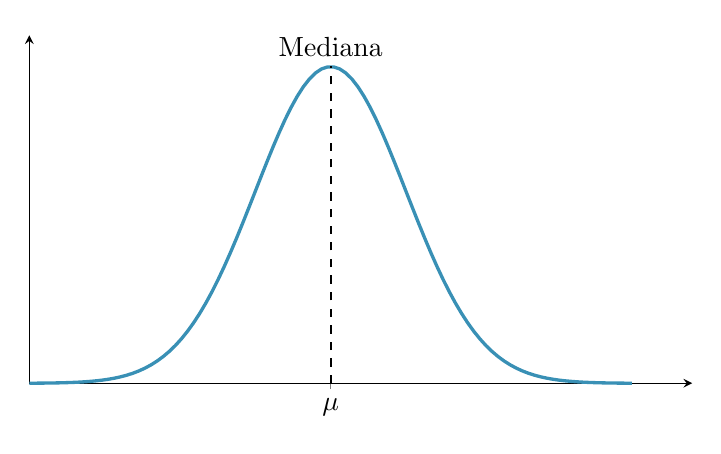
\begin{tikzpicture}
    \begin{axis}[
        no marks, 
        domain=-4:4, 
        samples=100,
        axis lines=left, 
        xlabel={}, ylabel={},
        every axis y label/.style={at=(current axis.above origin),anchor=south},
        every axis x label/.style={at=(current axis.right of origin),anchor=west},
        height=6cm, width=10cm,
        xtick={0}, 
        xticklabels={$\mu$}, % Indica la media/mediana
        ytick=\empty, 
        enlargelimits=upper,
        clip=false
        ]
        
        % Dibujo de la campana de Gauss
        \addplot [very thick, cyan!70!black] {exp(-x^2/2) / sqrt(2*pi)};
        
        % Línea discontinua en la mediana
        \draw [dashed, thick] (axis cs:0,0) -- (axis cs:0,0.4);
        
        % Opcional: etiqueta sobre la línea
        \node[above] at (axis cs:0,0.4) {Mediana};
        
    \end{axis}
    \end{tikzpicture}
    \caption{Distribución Normal con indicación de la mediana ($\mu$).}
    \label{fig:distribucion_normal}
\end{figure}
\begin{description}
    \item[¿Unicidad?] Si consideramos un ejemplo donde tengamos $a<b$ con $a,b\in \R$ tales que $P(X \leq a) = P(X \geq b) = 1/2$ y $P(a < X < b) = 0$, entonces cualquier valor $\mu \in [a,b]$ es una mediana de $X$, por lo que la mediana no es única en este caso. \\
    \noindent
    Para entender mejor esta demostración veremos un caso más concreto, suponiendo que \mbox{$X=-\mathbbm{1}_{A} + \mathbbm{1}_{A^c}$} con $P(A) = P(A^c) = 1/2$. En este caso, tenemos que $P(X \leq -1) = P(X \geq 1) = 1/2$ y $P(-1 < X < 1) = 0$, por lo que cualquier valor $\mu \in [-1,1]$ es una mediana de $X$, y por tanto la mediana no es única. \\
    \noindent
    Podemos ver una representación gráfica de este caso en la Figura \ref{fig:cdf_escalonada}, donde la función de distribución acumulada $F_X$ tiene una meseta en el intervalo $[-1,1]$, y cualquier valor en ese intervalo cumple las condiciones para ser mediana (hemos incluido el 1, pues también cumple las condiciones para ser mediana).
    \item[¿Existencia?] Si consideramos la función de distribución acumulada $F_X:\R \to [0,1]$ definida como $F_X(x) = P(X \leq x)$, que es monótona creciente y continua por la derecha, entonces definimos el siguiente valor
    \begin{equation*}
        \mu = \inf \{ x \in \R : F_X(x)=P(X\leq x) \geq 1/2 \}
    \end{equation*}
    que está bien definido, es decir, el conjunto $\{x : F_X(x) \geq 1/2\}$ no es vacío y está limitado inferiormente, pues $F_X$ va desde 0 hasta 1. Veamos ahora que este valor $\mu$ es una mediana de $X$
    \begin{enumerate}[label=\arabic*)]
        \item Por definición de mínimo (en este caso ínfimo y mínimo son lo mismo, gracias a la continuidad por la derecha de $F_X$), tenemos que $P(X\leq \mu)=F_X(\mu) \geq 1/2$, por lo que se cumple la primera condición de la mediana
        \item Por otro lado, falta demostrar que $P(X \geq \mu) \geq 1/2$, para ellos buscaremos demostrar que $P(X < \mu) \leq 1/2$, y por tanto tendríamos
        \begin{equation*}
            P(X \geq \mu) = 1 - P(X < \mu) \geq 1 - \dfrac{1}{2} = \dfrac{1}{2}
        \end{equation*}
        Para demostrar lo querido, usando la definición de ínfimo, sabemos que no hay $v< \mu$ con $F_X(v) \geq 1/2$, por lo que
        \begin{equation*}
            \forall v < \mu, \quad P(X \leq v) = F_X(v) < 1/2 
        \end{equation*}
        entonces $\lim_{v \to \mu} F_X(v) \leq 1/2$, y por la continuidad por la derecha de $F_X$, tenemos que $\lim\limits_{v \to \mu} F_X(v)=P(X < \mu)  \leq 1/2$, como queríamos demostrar.
    \end{enumerate}
\end{description}

\begin{figure}
    \centering
    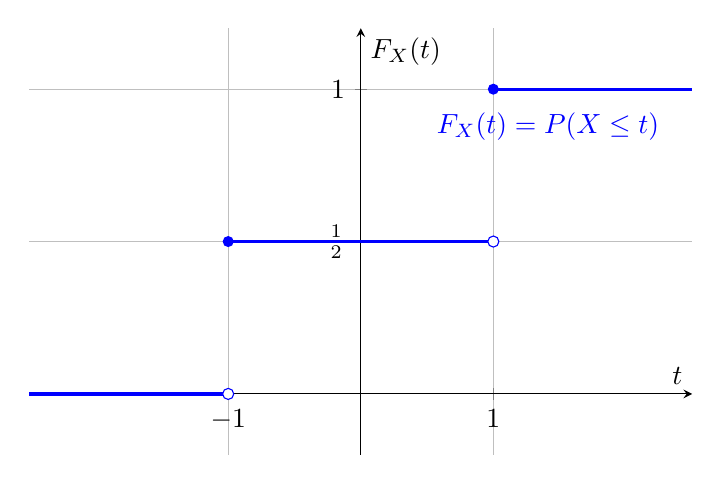
\begin{tikzpicture}
    \begin{axis}[
        axis lines=middle,
        grid=both,
        inner axis line style={=>},
        xlabel={$t$},
        ylabel={$F_X(t)$},
        ymin=-0.2, ymax=1.2,
        xmin=-2.5, xmax=2.5,
        ytick={0, 0.5, 1},
        yticklabels={0, $\frac{1}{2}$, 1},
        xtick={-1, 0, 1},
        height=7cm, width=10cm,
        clip=false
    ]
        % Texto de la función
        \node[blue, anchor=south west] at (axis cs: 0.5, 0.8) {$F_X(t) = P(X \leq t)$};

        % Tramo 1: de -infinito a -1 (valor 0)
        \draw[very thick, blue] (axis cs:-2.5, 0) -- (axis cs:-1, 0);
        \draw[blue, fill=white] (axis cs:-1, 0) circle (2pt);

        % Tramo 2: de -1 a 1 (valor 1/2)
        \draw[very thick, blue] (axis cs:-1, 0.5) -- (axis cs:1, 0.5);
        \fill[blue] (axis cs:-1, 0.5) circle (2pt);
        \draw[blue, fill=white] (axis cs:1, 0.5) circle (2pt);

        % Tramo 3: de 1 a infinito (valor 1)
        \draw[very thick, blue] (axis cs:1, 1) -- (axis cs:2.5, 1);
        \fill[blue] (axis cs:1, 1) circle (2pt);      
    \end{axis}
    \end{tikzpicture}
    \caption{Representación de la función de distribución acumulativa escalonada.}
    \label{fig:cdf_escalonada}
\end{figure}

\section{Leggi dei grandi numeri}


\begin{definicion}[Convergenza in probabilità]
    Sea $\{X_n\}_{n\in \bb{N}}$ una sucesión de variables aleatorias definidas sobre el mismo espacio de probabilidad $(\Omega, \mathcal{F}, P)$. Decimos que la sucesión \tbf{converge en probabilidad} a una variable aleatoria $X$, notado por $\{X_n\} \xrightarrow{P} X$, si:
    \begin{equation*}
        \forall \veps \in \bb{R}^+,\qquad \lim_{n\to \infty} P\left[|X_n - X| \geq \veps\right] = 0
    \end{equation*}
\end{definicion}

\begin{definicion}[Convergenza quasi certa]
    Sea $\{X_n\}_{n\in \bb{N}}$ una sucesión de variables aleatorias definidas sobre el mismo espacio de probabilidad $(\Omega, \mathcal, P)$. Decimos que la sucesión \tbf{converge casi seguramente} a una variable aleatoria $X$, que notaremos por $\{X_n\} \xrightarrow{c.s.} X$, si:
    \begin{equation*}
        P\left[\lim_{n\to \infty} X_n = X\right] = 1
    \end{equation*}
    Análogamente, usando la probabilidad en $(\Omega, \mathcal{F}, P)$, se tiene que:
    \begin{equation*}
        P\left[\omega\in \Omega\mid \lim_{n\to \infty} X_n(\omega) = X(\omega)\right] = 1
    \end{equation*}
\end{definicion}

\begin{prop}
    Sea $\{X_n\}_{n\in \bb{N}}$ una sucesión de variables aleatorias definidas sobre el mismo espacio de probabilidad $(\Omega, \mathcal{F}, P)$, entonces
    \begin{equation*}
        \{X_n\} \xrightarrow{c.s.} X \Longrightarrow \{X_n\} \xrightarrow{P} X 
    \end{equation*}
    \begin{proof}
        % //TODO: copiar de apuntes Jesus y Cristian
        % //TODO: entender
    \end{proof}
\end{prop}
\begin{observacion}
    La convergencia en probabilidad no implica la convergencia casi segura.
    % //TODO: copiar de apuntes de jesus y Cristian
    % //TODO: entender
\end{observacion}
\begin{prop}
    Sea $\{X_n\}_{n\in \bb{N}}$ una sucesión de variables aleatorias definidas sobre el mismo espacio de probabilidad $(\Omega, \mathcal{F}, P)$. Si la sucesión converge en probabilidad, entonces 
    \begin{equation*}
        \exists \text{ subsucesión } (n_j) \text{ tal que } \{X_{n_j}\} \xrightarrow{c.s.} X
    \end{equation*}
\end{prop}

\begin{teo}[Legge dei grandi numeri debole]
    Sea $(X_i)_{i\geq 1}$ una sucesión de variables aleatorias tales que
    \begin{itemize}
        \item $\E[|X_i|^2] < \infty$ para todo $i\geq 1$, es decir, $X_i \in \mathcal{L}^2(P)$.omega
        \item $Cov(X_i, X_j) = 0$ para todo $i\neq j$, es decir, las variables aleatorias son no correladas dos a dos (por ejemplo, independientes).
        \item $\sup\limits_{i\geq 1} Var(X_i) < \infty$, es decir, las varianzas están acotadas.
    \end{itemize}
    Entonces
    \begin{equation*}
        \forall \varepsilon > 0 \quad \lim_{n\to \infty}P\left( \left| \dfrac{1}{n} \sum_{i=1}^n (X_i - \E[X_i]) \right| \geq \varepsilon \right) = 0 \quad \text{es decir} \quad \dfrac{1}{n} \sum_{i=1}^n (X_i - \E[X_i]) \xrightarrow{P} 0
    \end{equation*}
    De hecho, si $\E[X_i] = n$ para todo $i\geq 1$, entonces
    \begin{equation*}
        \lim_{n\to \infty}P\left( \left| \dfrac{1}{n} \sum_{i=1}^n (X_i - n) \right| \geq \varepsilon \right) = 0 \quad \forall \varepsilon > 0
    \end{equation*}
    \begin{proof}
        % // TODO: copiar demostración de apuntes de Jesus y Cristian
    \end{proof}
\end{teo}

\begin{teo}[Versione più generale]
    Sea $(X_i)_{i\geq 1}$ una sucesión de variables aleatorias independientes dos a dos e idénticamente distribuidas en $\mathcal{L}^1(P)$, entonces
    \begin{equation*}
        \dfrac{1}{n} \sum_{i=1}^n X_i \xrightarrow{P} \E[X_1]
    \end{equation*}
\end{teo}

\begin{ejemplo}
    Para el caso del lanzamiento de una moneda justa, tenemos la secuencia de variables aleatorias $(X_i)_{i\geq 1}$ donde la v.a. $X_i$ representa el resultado del $i-$ésimo lanzamiento. Tenemos entonces
    \begin{equation*}
        \lim_{n\to \infty} \dfrac{1}{n} \sum_{i=1}^n X_i = p \in ]0,1[ \quad \text{casi seguro}
    \end{equation*}
    donde $\E[X_1] = p$.
\end{ejemplo}

\begin{observacion}
    La LGN débil es demasiado débil para poder capturar este tipo de convergencias.
\end{observacion}

\begin{lema}[Lemma di Borel-Cantelli]
    Sea $(A_n)_{n\in \N}$ una sucesión de eventos en un espacio de probabilidad $(\Omega, \mathcal{F}, P)$, y sea
    \begin{equation*}
        A=\bigcap_{k\geq 1} \bigcup_{n=k}^{\infty} A_n = \{\omega \in \Omega : \omega \in A_k \text{ para k valores } \infty \text{ de } k\}
    \end{equation*}
    entonces
    \begin{equation*}
        \text{ si } \sum_{n=1}^{\infty} P(A_n) < \infty \implies P(A) = 0
    \end{equation*}
    \begin{proof}
        % //TODO: copiar de apuntes de Jesus 
    \end{proof}
\end{lema}

\begin{coro}
    Sea $(\Omega, \mathcal{F}, P)$ un espacio de probabilidad y $\{E_n\}_{n \in \mathbb{N}}$ una sucesión de eventos en $\mathcal{F}$. Si la suma de las probabilidades de estos eventos es finita
    $$\sum_{n=1}^{\infty} P(E_n) < \infty$$
    Entonces, la probabilidad de que ocurran infinitos de estos eventos es cero
    $$P(\limsup_{n \to \infty} E_n) = 0$$
\end{coro}

\begin{teo}[Legge dei grandi numeri forte]
    Sea $(X_i)_{i\geq 1}$ una sucesión de variables aleatorias tales que
    \begin{itemize}
        \item $\E[|X_i|^2] < \infty$ para todo $i\geq 1$, es decir, $X_i \in \mathcal{L}^2(P)$.
        \item $Cov(X_i, X_j) = 0$ para todo $i\neq j$, es decir, las variables aleatorias son no correladas dos a dos (por ejemplo, independientes).
        \item $\sup\limits_{i\geq 1} Var(X_i) < \infty$, es decir, las varianzas están acotadas.
    \end{itemize}
    Entonces
    \begin{equation*}
        P\left( \lim_{n\to \infty} \dfrac{1}{n} \sum_{i=1}^n (X_i - \E[X_i]) = 0 \right) = 1 \quad \text{es decir} \quad \dfrac{1}{n} \sum_{i=1}^n (X_i - \E[X_i]) \xrightarrow{c.s.} 0
    \end{equation*}
    \begin{proof}
        % //TODO: copiar de apuntes de Jesus
        % //TODO: entender
    \end{proof}
\end{teo}

\begin{observacion}
    Es importante destacar que el conjunto 
    $$\lim_{n\to \infty} \dfrac{1}{n} \sum_{i=1}^n (X_i - \E[X_i]) = 0 $$
    es realmente los $\omega \in \Omega$ tales que $\lim\limits_{n\to \infty} \dfrac{1}{n} \sum\limits_{i=1}^n (X_i(\omega) - \E[X_i]) = 0$, y de este conjunto de $\omega$'s tenemos que la probabilidad es 1.
\end{observacion}

\begin{coro}
    Sea $(X_i)_{i\geq 1}$ una sucesión de variables aleatorias idénticamente distribuidas y dos a dos no correladas en $\mathcal{L}^2(P)$ con $v:=\sup_{i\geq 1} Var(X_i) < \infty$, entonces
    \begin{equation*}
        \dfrac{1}{n} \sum_{i=1}^n X_i \xrightarrow{c.s.} \E[X_1]
    \end{equation*}
\end{coro}

\noindent
En el resultado anterior, la hipótesis de que las variables aleatorias son idénticamente distribuidas es lo que nos permite afirmar que $\E[X_i] = \E[X_1]$ para todo $i\geq 1$.

\begin{prop}[Composición de sucesiones convergentes c.s.]
    La composición de sucesiones convergentes casi seguramente también converge casi seguramente, es decir, si $\{X_n\} \xrightarrow{c.s.} X$ y $\{Y_n\} \xrightarrow{c.s.} Y$, entonces
    \begin{equation*}
        \{X_n + Y_n\} \xrightarrow{c.s.} X + Y \quad , \quad \{X_n Y_n\} \xrightarrow{c.s.} XY
    \end{equation*}
\end{prop}

\section{Teorema Central del Límite}
\noindent
En la sección anterior hemos visto que 
\begin{equation*}
    \lim_{n\to \infty} \dfrac{1}{n} \sum_{i=1}^n X_i = \E[X_1] \quad \text{c.s.}
\end{equation*}
bajo las condiciones 
\begin{itemize}
    \item $(X_i)_{i\geq 1}$ son variables aleatorias no correladas dos a dos e idénticamente distribuidas, es decir, $P(X_i\in A)$ no depende de $i$.
    \item $\E[|X_1|^2] < \infty$, indicado solo para $X_1$ ya que todas las demás variables aleatorias tienen la misma distribución.
\end{itemize}
donde si además nombramos $m = \E[X_1]$, nos podemos preguntar cuál es el número $1-\alpha$ más grande tal que
\begin{equation*}
    \lim_{n\to \infty} n^{1-\alpha} \left( \dfrac{1}{n} \sum_{i=1}^n X_i - m \right) = 0 \quad \text{c.s.}
\end{equation*}
Más adelante, veremos que el número más grande es $\alpha = 1/2$ gracias al Teorema Central del Límite, pero primero veremos unos enunciados que nos ayudarán a entender mejor este teorema.

\begin{definicion}[Convergenza in distribuzione]
    Sea $\{X_n\}_{n\in \bb{N}}$ una sucesión de variables aleatorias definidas sobre el mismo espacio de probabilidad $(\Omega, \mathcal{F}, P)$. Decimos que la sucesión \tbf{converge en distribución} a una variable aleatoria $X$, notado por $\{X_n\} \xrightarrow{d} X$, si:
    \begin{equation*}
        \lim_{n\to \infty} F_{X_n}(t) = F_X(t) \quad \forall t \in C(F_X)
    \end{equation*}
    donde $F_{X_n}$ y $F_X$ son las funciones de distribución acumulada de $X_n$ y $X$ respectivamente, y $C(F_X)$ es el conjunto de puntos de continuidad de $F_X$. \\
    \noindent
    Además, se dice que la sucesión \tbf{converge en distribución a una medida} $\mu$ de probabilidad en $(\R, \mathcal{B}(\R))$, notado por $\{X_n\} \xrightarrow{d} \mu$, si
    \begin{equation*}
        \lim_{n\to \infty} F_{X_n}(t) = \mu(]-\infty, t]) \quad \forall t \in C(\mu)
    \end{equation*}
    donde $C(\mu)$ es el conjunto de puntos de continuidad de la función $\mu(]-\infty, t])$.
\end{definicion}

\begin{notacion}
    A veces en lugar de hablar de \textit{convergencia en distribución} a una variable aleatoria $X$, se habla de \underline{convergencia en ley} y se nota como $\{X_n\} \xrightarrow{L} X$.
\end{notacion}

\begin{lema}[Caracterización de la convergencia en la distribución.]
    Sea $\{X_n\}_{n\in \bb{N}}$ una sucesión de variables aleatorias definidas sobre el mismo espacio de probabilidad $(\Omega, \mathcal{F}, P)$, las siguientes afirmaciones son equivalentes:
    \begin{enumerate}[label=\arabic*)]
        \item $X_n \xrightarrow{d} X$
        \item $\E[f(X_n)] \to \E[f(X)] \quad \forall f:\R \to \R$ continua y acotada.
    \end{enumerate}
    Si $F_X$ es continua en $\R$, entonces la siguiente afirmación también es equivalente
    \begin{equation*}
        \lim_{n\to \infty} \sup_{c\in \R} |F_{X_n}(c)-F_X(c)|=0
    \end{equation*}
    es decir, $F_{X_n}$ converge uniformemente a $F_X$.
    \begin{proof}
        Solo demostraremos la segunda parte del enunciado.
        % //TODO: copiar demostración de Jesus
    \end{proof}
\end{lema}

\begin{observacion}
    Recordemos que $\E[f(X_n)]= \int_{\R}f(z)d\mu_n(z)$ donde $\mu_n(A)=P(X_n\in A)$.
\end{observacion}

\begin{teo}[Teorema Central del Límite]
    Sea $(X_i)_{i\geq 1}$ una sucesión de variables aleatorias independientes e idénticamente distribuidas en $\mathcal{L}^2(P)$, es decir, tales que $\E[|X_i|^2] < \infty \ \forall i$. Si nombramos $m = \E[X_i]$ y $v = Var(X_i)$, entonces
    \begin{equation*}
        \dfrac{1}{\sqrt{n}}\sum\limits_{i=1}^n \dfrac{X_i - m}{\sqrt{v}} \xrightarrow{d} Z \sim N(0,1)
    \end{equation*}
    donde $N(0,1)$ es la distribución normal estándar con media 0 y varianza 1, es decir,
    \begin{equation*}
        Z(]-\infty, t]) = \dfrac{1}{\sqrt{2\pi}} \int_{-\infty}^t e^{-\frac{x^2}{2}} \, dx=\Phi(t) \quad \forall t \in \R
    \end{equation*}
    Además, como la función de distribución de la normal $\Phi$ es continua tenemos que 
    \begin{equation*}
        \lim_{n\to \infty} \sup_{c\in \R}|F_{S_n^*}(c)- \Phi(c)|=0
    \end{equation*}
    dove $S_n^* = \dfrac{1}{\sqrt{n}}\sum\limits_{i=1}^n\dfrac{ X_i - m}{\sqrt{v}}$
    \begin{proof}
        % //TODO: copiar de apuntes de Jesus y Cristian
        % //TODO: entender
    \end{proof}
\end{teo}

\begin{coro}
    Sean $X,Y$ distribuciones gaussianas independientes con media 0 y varianza 1, entonces
    \begin{equation*}
        \mu_{\frac{X+Y}{\sqrt{2}}} \sim N(0,1)
    \end{equation*}
    De hecho, en general dadas $X,Y$ variables aleatorias independientes con funciones de densidad $f_X, f_Y$, entonces la función de densidad de $X+Y$ es
    \begin{equation*}
        f_{X+Y}(t)=\int_{\R} f_X(t - s) f_Y(s) \, ds
    \end{equation*}
\end{coro}

\noindent 
Dado el Teorema Central del Límite, vemos que este teorema parece ser una ley universal para todas las v.a. i.i.d. en $\mathcal{L}^2(P)$, por lo que es lógico preguntarse entonces que si de verdad funciona este teorema debería hacerlo también para v.a. que sigan una distribución normal de media 0 y varianza 1. A continuación, veremos un ejemplo que confirma esta hipótesis.

\begin{ejemplo}
    Sea $(X_i)_{i\geq 1}$ una sucesión de v.a. independientes e idénticamente distribuidas con distribución $N(0,1)$, sabemos que su suma también sigue una distribución normal por su propiedad de reproductividad, es decir,
    \begin{equation*}
        S_n = \sum_{i=1}^n X_i \sim N(0,n)
    \end{equation*}
    por lo que si normalizamos $S_n$ como bien dice el Teorema Central del Límite, tenemos que
    \begin{equation*}
        S_n^* = \dfrac{S_n - 0}{\sqrt{n}} = \dfrac{1}{\sqrt{n}} \sum_{i=1}^n X_i \sim N(0,1)
    \end{equation*}
    y por tanto $S_n^*$ ya tiene la distribución límite que predice el Teorema Central del Límite. Hemos visto entonces, que como bien se preveía, este teorema funciona de forma general, incluso en el caso más obvio de v.a. con distribución normal.
\end{ejemplo}

